%===================================================
%================== DOCUMENT CLASS
%===================================================
\documentclass[runningheads,11pt,a4paper,english,llncs]{Misc/llncs}

%===================================================
%================== PACKAGES
%===================================================
%------------------------------------------------------------------------
% TeX and LaTeX macros
%------------------------------------------------------------------------
%
% In math formulas we use italic instead of mathitalic
%
\makeatletter
% ~ gives a \; space in math mode
\def~{\ifmmode\;\else\penalty\@M\ \fi}
%  Italic in mathematical formulas
\def\@setmcodes#1#2#3{{\count0=#1 \count1=#3
  \loop \global\mathcode\count0=\count1 \ifnum \count0<#2
  \advance\count0 by1 \advance\count1 by1 \repeat}}
\DeclareSymbolFont{italic}{OT1}{\rmdefault}{m}{it}
\let\mathit\undefined
\DeclareSymbolFontAlphabet{\mathit}{italic}
\edef\@tempa{\hexnumber@\symitalic}
\@setmcodes{`A}{`Z}{"7\@tempa41}
\@setmcodes{`a}{`z}{"7\@tempa61}
\makeatother
%
% \begin{asm} ... \end{asm}
%
\newdimen\asmindent     
\asmindent=\parindent
\newcount\asmi
\def\inc{\global\advance\asmi by 1}
\def\dec{\global\advance\asmi by-1}
\def\nl{{}$\par\hangindent\asmi em
  \noindent\kern\asmi em\ignorespaces$} 
\def\asmskip{{}$\par\smallskip\hangindent\asmi em
  \noindent\kern\asmi em\ignorespaces$}

%%%%%%%%%%%%%%%%%%%%%%%%%%%
\def\asm{\global\asmi=0 
 \def\+{\inc\nl}
 \def\-{\dec\nl}
 \def\\{\nl}
 %%% Added by Paolo 2018-06-25:
 \setlength{\parskip}{0pt}
 %%%
 \begin{trivlist}\item[]\leftskip=\asmindent\relax$}
%%%%%%%%%%%%%%%%%%%%%%%%%%%

\def\endasm{$\end{trivlist}}
%\mathindent=\asmindent
%
% \begin{asmarray}
%    f(s_1) & := t_1 \\
%    f(s_2) & := t_2 
% \end{asmarray}
%
\def\asmarray{\begin{array}[t]{@{}l@{\;}l@{\;}l@{}}}
\def\endasmarray{\end{array}}
%
%
%
\def\asmcomment#1{\quad\hbox{// #1}}
%
%  \begin{subasm} ... \end{subasm}
%
\newcount\asmii
\def\subasm{\vtop\bgroup\asmii=0\normalbaselines
 \def\nl##1{$\egroup\advance\asmii by##1\relax\hbox\bgroup\hskip\asmii em$}
 \def\\{\nl{0}}
 \def\+{\nl{1}}
 \def\-{\nl{-1}}
 \hbox\bgroup\hskip\asmii em$}
\def\endsubasm{$\egroup\egroup}
%
% Keywords in ASM code
%
\def\ASM#1{\hbox{\sc#1}}        % rule names and macros
\def\ASMIND#1{\ASM{#1}\index{#1@{\sc#1}}}
\def\AWAIT   {\mathrel{\mathbf{await}}}
\def\AND     {\mathrel{\mathbf{and}}}
\def\CASE    {\mathrel{\mathbf{case}}}
\def\CHOOSE  {\mathrel{\mathbf{choose}}}
\def\CREATE  {\mathrel{\mathbf{create}}}
\def\NEW  {\mathrel{\mathbf{new}}}
\def\DO      {\mathrel{\mathbf{do}}}
\def\ELSE    {\mathrel{\mathbf{else}}}
\def\ELSEIF  {\mathrel{\mathbf{elseif}}}
\def\FORALL  {\mathrel{\mathbf{forall}}}
\def\FORSOME  {\mathrel{\mathbf{forsome}}}
\def\FOREACH  {\mathrel{\mathbf{foreach}}}
\def\THEREISNO  {\mathrel{\mathbf{thereisno}}}
\def\FROM  {\mathrel{\mathbf{from\colon}}}
\def\FOR  {\mathrel{\mathbf{for\colon}}}
\def\TO  {\mathrel{\mathbf{to\colon}}}
\def\IF      {\mathrel{\mathbf{if}}}
\def\IFF      {\mathrel{\mathbf{iff}}}
\def\IMPORT  {\mathrel{\mathbf{import}}}
\def\IN      {\mathrel{\mathbf{in}}}
\def\LET     {\mathrel{\mathbf{let}}}
\def\SELF    {\mathrel{\mathbf{self}}}
\def\MATCH    {\mathrel{\textbf{match}}}
\def\NOT     {\mathrel{\mathbf{not}}}
\def\OF      {\mathrel{\mathbf{of}}}
\def\OR      {\mathrel{\mathbf{or}}}
\def\PAR     {\mathrel{\mathbf{par}}}
\def\SEQ     {\mathrel{\mathbf{seq}}}
\def\SKIP    {\mathrel{\mathbf{skip}}}
\def\THEN    {\mathrel{\mathbf{then}}}
\def\WHERE   {\mathrel{\mathbf{where}}}
\def\WHILE   {\mathrel{\mathbf{while}}}
\def\UNDEF   {\mathrel{\mathbf{undef}}}
\def\UNTIL   {\mathrel{\mathbf{until}}}
\def\WHEN   {\mathrel{\mathbf{when}}}
\def\WITH    {\mathrel{\mathbf{with}}}
\def\STEP    {\mathrel{\mathbf{step}}}
\def\STEPWISE    {\mathrel{\mathbf{stepwise}}}
\def\SEQ    {\mathrel{\mathbf{seq}}}
\def\RESULT  {\mathrel{\mathbf{result}}}
\def\CALL  {\mathrel{\mathbf{Call}}}
\def\LOCAL    {\mathrel{\mathbf{local}}}
\def\ADDGUARD {\mathrel{\mathbf{addGuard}}}
\def\ADDUPD   {\mathrel{\mathbf{addUpd}}}
\def\ADDRULE  {\mathrel{\mathbf{addRule}}}
\def\MINUSRULE  {\mathrel{\mathbf{minusRule}}}
%\def\TO      {\mathrel{\mathbf{to}}}
%
% Including figures
%
\def\includefig#1#2{\centering\medskip
  \includegraphics[scale=#1]{fig/#2}
  \medskip}
%
% References to paragraphs in the ECMA standard for C#
%
\def\ecma#1{\cite[\S#1]{ecma334}}
%
%  Environments for definitions and theorems
%
%\theorembodyfont{\rm}
%\newtheorem{definition}[subsection]{Definition}
%\newtheorem{lemma}[subsection]{Lemma}
%\newtheorem{theorem}[subsection]{Theorem}
%\newtheorem{proposition}[subsection]{Proposition}
%\newtheorem{corollary}[subsection]{Corollary}
%\newtheorem{example}[subsection]{Example}
%\newtheorem{remark}[subsection]{Remark}
%\newtheorem{constraint}[subsection]{Constraint}
\def\proof{\trivlist\item[]{\bf Proof.}}
\def\endproof{$\Box$\endtrivlist}
%
% enumerate and itemize (smaller skips) from "latex.ltx"
%
\makeatletter
\def\enumerate{%
  \ifnum \@enumdepth >\thr@@\@toodeep\else
    \advance\@enumdepth\@ne
    \edef\@enumctr{enum\romannumeral\the\@enumdepth}%
      \expandafter
      \list
        \csname label\@enumctr\endcsname
        {\usecounter\@enumctr\def\makelabel##1{\hss\llap{##1}}
         \itemsep 0pt\parskip 0pt\parsep 0pt\topsep\smallskipamount}%
  \fi}
\def\itemize{%
  \ifnum \@itemdepth >\thr@@\@toodeep\else
    \advance\@itemdepth\@ne
    \edef\@itemitem{labelitem\romannumeral\the\@itemdepth}%
    \expandafter
    \list
      \csname\@itemitem\endcsname
      {\def\makelabel##1{\hss\llap{##1}}
       \itemsep 0pt\parskip 0pt\parsep 0pt\topsep\smallskipamount}%
  \fi}
\makeatother
%
% items in itemize
%
\def\bull{\vrule height .9ex width .8ex depth -.1ex}
\def\labelitemi{\bull}
%
%
%
\def\cs#1{C\#$_{\mathcal{#1}}$}
\def\lang#1{L$_{\mathcal{#1}}$}
%
% Positions
%
\def\pos#1{{}^{#1}}
\def\termPos{\blacktriangleright}
\def\cursor{\pos{\termPos}}
%
%
%
\def\sup{\hbox{sup}}
\def\c#1{\texttt{#1}}           % code
\def\N#1{\textit{#1}}           % non terminal symbols
\def\T#1{\hbox{`\texttt{#1}'}}  % terminal symbols
\def\A#1{\hbox{\sc#1}}          % ASM rules
\def\D#1{#1}                    % dynamic functions
\def\U#1{#1}                    % universes
\def\C#1{#1}                    % constructors
\def\rdef{\equiv}
\def\lbr{\c{\char`\{}}
\def\rbr{\c{\char`\}}}
\def\mb{\hbox{::}}
\def\map#1#2{\textbf{Map from}~#1~\textbf{to}~#2}
\def\cat{\cdot}
\def\adots{\mathinner{\ldotp\ldotp}}
%
%
% macros.tex ends here

\usepackage{bera}% optional: just to have a nice mono-spaced font
\usepackage{listings}
\usepackage{xcolor}

\colorlet{punct}{red!60!black}
\definecolor{background}{HTML}{FFFFFF}
\definecolor{delim}{RGB}{20,105,176}
\colorlet{numb}{magenta!60!black}

\lstdefinelanguage{json}{
    basicstyle=\normalfont\ttfamily,
    commentstyle=\color{eclipseStrings}, % style of comment
    stringstyle=\color{eclipseKeywords}, % style of strings
    numbers=left,
    numberstyle=\scriptsize,
    stepnumber=1,
    numbersep=8pt,
    showstringspaces=false,
    breaklines=true,
    frame=lines,
	string=[s]{"}{"},
    comment=[l]{:\ "},
    morecomment=[l]{:"},
}
\usepackage{bera}% optional: just to have a nice mono-spaced font
\usepackage{listings}
\usepackage{xcolor}
\definecolor{eclipseStrings}{RGB}{42,0.0,255}
\definecolor{eclipseComment}{RGB}{63,127,95}
\definecolor{eclipseKeywords}{RGB}{127,0,85}

\lstdefinelanguage{bsl}{
    % list of keywords
  	morekeywords={
		universe, controlled, location,
    	if, then, endif,
	    while,    	
    	send,
    	or, and, to, in, do, with,
		CoreASIM,
		policy,
		use,
		init,
		rule,
		scheduling, schedule,
    	subject,
    	forall,
    	choose,
		derived,
    	skip, undef,
    	case, endcase, 
    	seq, endseq, par, endpar, block, endblock, next,
    	createASIM, destroyASIM, initializedBy, withProgram, andPolicy,
  	},
  	sensitive=true, % keywords are not case-sensitive
  	morecomment=[l]{//}, % l is for line comment
  	morecomment=[s]{/*}{*/}, % s is for start and end delimiter
  	morestring=[b]" % defines that strings are enclosed in double quotes
}

% Set Language
\lstset{
  language={bsl},
  basicstyle=\normalfont\ttfamily, % Global Code Style
  captionpos=b, % Position of the Caption (t for top, b for bottom)
  extendedchars=true, % Allows 256 instead of 128 ASCII characters
  tabsize=2, % number of spaces indented when discovering a tab 
  columns=fixed, % make all characters equal width
  keepspaces=true, % does not ignore spaces to fit width, convert tabs to spaces
  showstringspaces=false, % lets spaces in strings appear as real spaces
  breaklines=true, % wrap lines if they don't fit
  commentstyle=\color{eclipseComment}, % style of comments
  keywordstyle=\color{eclipseKeywords}, % style of keywords
  stringstyle=\color{eclipseStrings}, % style of strings
}

\lstdefinelanguage{bsl_lst}{
    % list of keywords
  	morekeywords={
		universe, controlled, location,
    	if, then, endif,
	    while,    	
    	send,
    	or, and, to, in, do, with,
		CoreASIM,
		policy,
		use,
		init,
		rule,
		scheduling, schedule,
    	subject,
    	forall,
    	choose,
		derived,
    	skip, undef,
    	case, endcase, of,
    	seq, endseq, par, endpar, block, endblock, next,
    	createASIM, destroyASIM, initializedBy, withProgram, andPolicy,
  	},
  	sensitive=true, % keywords are not case-sensitive
  	morecomment=[l]{//}, % l is for line comment
  	morecomment=[s]{/*}{*/}, % s is for start and end delimiter
  	morestring=[b]", % defines that strings are enclosed in double quotes
  	frame=lines,
  	basicstyle=\normalfont\ttfamily, % Global Code Style
	basicstyle=\normalfont\ttfamily, % Global Code Style
    captionpos=b, % Position of the Caption (t for top, b for bottom)
    extendedchars=true, % Allows 256 instead of 128 ASCII characters
    tabsize=2, % number of spaces indented when discovering a tab 
    columns=fixed, % make all characters equal width
    keepspaces=true, % does not ignore spaces to fit width, convert tabs to spaces
    showstringspaces=false, % lets spaces in strings appear as real spaces
    breaklines=true, % wrap lines if they don't fit
    numbers=left, % show line numbers at the left
    numberstyle=\tiny\ttfamily, % style of the line numbers
    commentstyle=\color{eclipseComment}, % style of comments
    keywordstyle=\color{eclipseKeywords}, % style of keywords
    stringstyle=\color{eclipseStrings}, % style of strings
}
\usepackage{bera}% optional: just to have a nice mono-spaced font
\usepackage{listings}
\usepackage{xcolor}

\colorlet{punct}{red!60!black}
\definecolor{background}{HTML}{FFFFFF}
\definecolor{delim}{RGB}{20,105,176}
\colorlet{numb}{magenta!60!black}

\lstdefinelanguage{yaml}{
    basicstyle=\normalfont\ttfamily,
    commentstyle=\color{eclipseStrings}, % style of comment
    stringstyle=\color{eclipseKeywords}, % style of strings
    numbers=left,
    numberstyle=\scriptsize,
    stepnumber=1,
    numbersep=8pt,
    showstringspaces=false,
    breaklines=true,
    frame=lines,
	string=[s]{"}{"},
    comment=[l]{\#},
}
\usepackage{etex}
\reserveinserts{28}
\newcommand{\todo}[1]{
 \noindent{\newline \color{red}
 \framebox[\textwidth][t]{%
  \parbox[t]{0.9\textwidth}{\textcolor{red}{TODO: #1}}                                                                                     
}}}
\usepackage{listings}
\lstset{
  basicstyle=\ttfamily,
  columns=fullflexible,
  breaklines=true,
  postbreak=\mbox{\textcolor{red}{$\hookrightarrow$}\space},
}
\usepackage{graphicx}
\usepackage{acronym}
\usepackage{ifthen}
\usepackage{substr}
\usepackage{color}
\usepackage{fixltx2e}
\usepackage[left=2cm, top=2cm, right=2cm, bottom=2cm]{geometry}
%\usepackage{subfigure}
\usepackage{array}  
\usepackage[figuresright]{rotating}          
\usepackage{url}
\usepackage{tikz}
\usetikzlibrary{trees}
%\usepackage{enumerate}
\usepackage[shortlabels]{enumitem}
\usepackage{epsfig}
\usepackage{colordvi}
\usepackage{makeidx}
\usepackage{index}
\usepackage[absolute]{textpos}
\setlength{\TPHorizModule}{\paperwidth}
\setlength{\TPVertModule}{\TPHorizModule}
\textblockorigin{-6mm}{0mm}
\usepackage[%
      breaklinks=true,%
      colorlinks=true,%           no frame around URL
      urlcolor=LINK_COLOR,%            no colors
      menucolor=LINK_COLOR,%           no colors
      linkcolor=LINK_COLOR,%           no colors
      pagecolor=LINK_COLOR,%           no colors
      bookmarks=true,%            tree-like TOC
      bookmarksopen=false,%       expanded when starting
      hyperfootnotes=true,%       no referencing of footnotes, does not compile
      citecolor=CITE_COLOR,%           black cites
      filecolor=black,%           black files%
      hyperindex=true,%
      hyperfigures=true%
]{hyperref}
\usepackage{bookmark}
\usepackage{booktabs}
\usepackage{dsfont}
\usepackage{wallpaper}
\usepackage{mathtools,cancel}
\usepackage{soul}
\usepackage{float}
\usepackage{setspace}
%\usepackage{morefloats}
%\usepackage{mdwlist}
\usepackage{amsmath,amssymb,amscd,diagrams,bm,amsfonts}
\let\proof\relax
\let\endproof\relax
\usepackage{amsthm}
\usepackage{tabularx, graphics, longtable, multirow, makecell}

%%%%%%% Added by Paolo 2018-03:
\usepackage[justification=centering]{caption}
\usepackage{eurosym}
%%%%%%%%%%%%%%%%%%%%%%

%\usepackage[title]{appendix}


%TIKZ
\usepackage{tikz}
\usepackage{tikz-cd}
\usetikzlibrary{trees,snakes}
\usetikzlibrary{arrows,automata}
\usetikzlibrary{matrix,arrows,positioning}
\usetikzlibrary{mindmap,backgrounds}
\usetikzlibrary{shapes}
\usepackage{verbatim} %for comment out some texts

%%%%%%%%%%%%%%%%%%%%%%%%%%%%%%%
%%%%%%%%%%%%%%%%%%%%% Egon's commands:
\usepackage{latexsym}
\ifx\pdfoutput\undefined
  \message{We are running LaTeX.} 
%PD  \usepackage[dvips]{graphicx}
%PD  \DeclareGraphicsExtensions{.eps}
%PD  \usepackage[hypertex,bookmarks=false]{hyperref}
\else
  \message{We are running PDFLaTeX.}
%PD  \usepackage[pdftex]{color}
%PD  \usepackage[pdftex]{graphicx}
%PD\DeclareGraphicsExtensions{.jpg,.pdf}
%PD  \DeclareGraphicsExtensions{.pdf}
%PD  \usepackage[pdftex,bookmarks=false]{hyperref}
%PD  \hypersetup{colorlinks={true},
%PD            linkcolor={blue},
%PD            citecolor={blue},
%PD            urlcolor={blue},
%PD            plainpages={false}
%PD  }
\fi
%%%%%%%%%%%%%%%%%%%%%%%%%%%%%%%
%%%%%%%%%%%%%%%%%%%%%%%%%%%%%%%

%===================================================
%================== THEOREMS
%===================================================
\theoremstyle{plain}
\newtheorem{thm}{Theorem}
\newtheorem{cor}[thm]{Corollary}
\newtheorem{lem}[thm]{Lemma}
\newtheorem{prop}[thm]{Proposition}
\newtheorem{defin}[thm]{Definition}
\newtheorem{rmrk}[thm]{Remark}

\allowdisplaybreaks


%===================================================
%================== COLOURS
%==================================================

\definecolor{green}{rgb}{0,0.6,0} 
\definecolor{gray}{rgb}{0.6,0.6,0.6} 
\definecolor{red}{rgb}{1,0,0} 
\definecolor{blue}{rgb}{0,0,1} 
\definecolor{purple}{rgb}{0.5,0,0.5} 
\definecolor{yellow}{rgb}{0.25,0.25,0} 
\definecolor{turquoise}{rgb}{0,0.5,0.5}
\definecolor{brown}{rgb}{0.6,0.2,0.1}

\definecolor{LINK_COLOR}{rgb}{0,0,0.7}
\definecolor{CITE_COLOR}{rgb}{0,0.5,0}
\definecolor{lightblue}{rgb}{0,0,1}
\definecolor{light-gray}{gray}{0.95}
\def\red#1{\textcolor[rgb]{1.0,0.0,0.0}{#1}}
\def\green#1{\textcolor[rgb]{0.0,0.8,0.1}{#1}}
\def\blue#1{\textcolor[rgb]{0.0,0.0,1.0}{#1}}

%===================================================
%================== LAYOUT
%===================================================
\parindent=0cm
%\setlength{\parskip}{1.0\baselineskip plus 0.5ex minus 0.2ex}
\abovecaptionskip=0cm
\hyphenpenalty=5000
\tolerance=1000 
\floatsep=1in
\allowdisplaybreaks
\def \constzeroindent {0cm}
\def \constfirstindent {0.5cm}
\def \constsecondindent {1cm}
\newenvironment{mycustomindent}[1]
{\setlength{\parindent}{#1}}
{\setlength{\parindent}{\constzeroindent}}
\newcommand{
	\firstindent}[1]{
	\begin{mycustomindent}{\constfirstindent}
	\begin{tabular}{@{}p{12cm}@{}}
	#1 \\
	\end{tabular}
	\end{mycustomindent}
}
\newcommand{
	\secondindent}[1]{
	\begin{mycustomindent}{\constsecondindent}
	\begin{tabular}{@{}p{12cm}@{}}
	#1 \\
	\end{tabular}
	\end{mycustomindent}
}
\newenvironment{packed_item1}{
\begin{itemize}[topsep=0pt, partopsep=0pt]
  \setlength{\itemsep}{5pt}
  \setlength{\parskip}{0pt}
  \setlength{\parsep}{0pt}
}{\end{itemize}}
\newenvironment{packed_item2}{
\begin{itemize}[topsep=0pt, partopsep=0pt]
  \setlength{\itemsep}{0pt}
  \setlength{\parskip}{0pt}
  \setlength{\parsep}{0pt}
}{\end{itemize}}
\newenvironment{packed_enumerate}{
\begin{enumerate}[topsep=0pt, partopsep=0pt]
  \setlength{\itemsep}{5pt}
  \setlength{\parskip}{0pt}
  \setlength{\parsep}{0pt}
}{\end{enumerate}}
% The following commands are to get rid of the extra space around section and subsection titles:
% Save the class definition of \subparagraph:
\let\llncssubparagraph\subparagraph
% Provide a definition to \subparagraph to keep titlesec happy:
\let\subparagraph\paragraph
\usepackage[compact]{titlesec}
\usepackage{dblfloatfix,caption,subcaption}
\titlespacing{\section}{0pt}{12pt}{*0}
\titlespacing{\subsection}{0pt}{6pt}{0pt}
\titlespacing{\subsubsection}{0pt}{6pt}{0pt}
% Force section numbering to follow chapter numbering:
\usepackage{chngcntr}
\counterwithin{section}{chapter}
\counterwithin{figure}{chapter}
%\counterwithin{theorem}{chapter}
%\counterwithin{lemma}{chapter}
%\counterwithin{definition}{chapter}
%%%%%%%%%%%%%%%%%%%%%%%%%%%%
% Allow line breaks in long list of citations that would extend into the margin:
\usepackage{breakcites}
%%%%%%%%%%%%%%%%%%%%%%%%%%%%%%%%%%%%%%

\usepackage{pdfpages}
\pagestyle{headings}

\renewcommand{\rightmark}{INTERLACE Project (Grant no.~754494)}
\renewcommand{\leftmark}{D3.1}
\setcounter{tocdepth}{2}

\usepackage{tocloft}
\setlength\cftparskip{0pt}
\setlength\cftbeforechapskip{12pt}

%\renewcommand{\cfttoctitlefont}{\normalfont\MakeUppercase}

\usepackage{abstract}
\renewcommand{\abstractnamefont}{\large \bfseries}
%\setlength{\abstitleskip}{-\absparindent}
\renewcommand{\abstractname}{Abstract}

\setlength{\parskip}{12pt}

\begin{document}
%===================================================
%================== TITLE
%===================================================

\thispagestyle{empty}
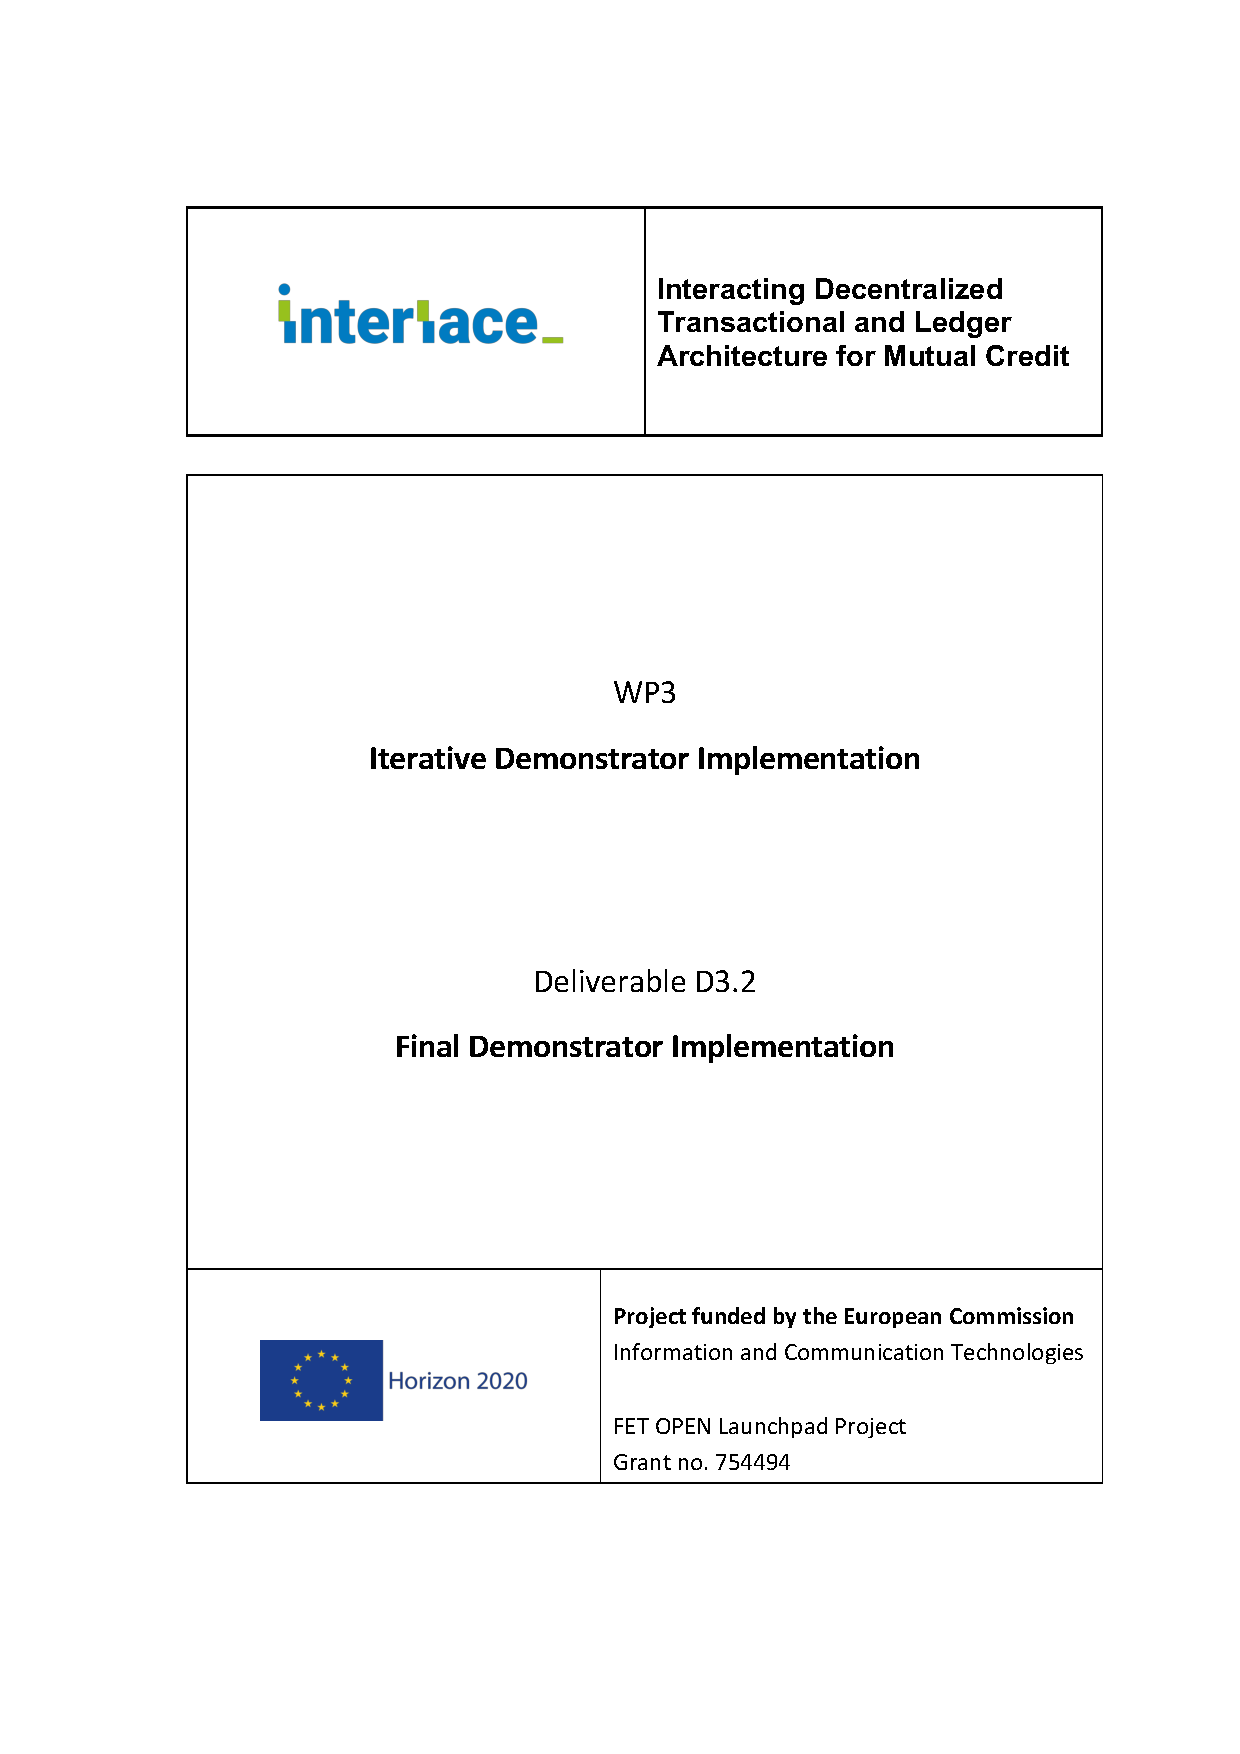
\includepdf[pages=-, scale=1.0]{Misc/Front}

%===================================================
%================== ABSTRACT
%===================================================
\thispagestyle{empty}

\begin{abstract}
\normalsize
This report describes the Hyperledger implementation of a part of the specification detailed in Delievarble D3.1: Requirements and Architecture Definition, as well as mechanisms used to ensure a stable and shared runtime environment and to guarantee testability and easy execution of the ASIM model of the business logic. The implementation is based on a refinement of the requirements that is detailed in this report, along with an updated formal specification, relative to the original ASIM definitions of D2.1, in the Appendix. Finally, a presentation of the runtime environment is given and discussed in the context of the future connection to the blockchain-based backend.
\end{abstract}

\newpage

%===================================================
%================== TABLE OF CONTENTS
%===================================================
\tableofcontents


%===================================================
%================== CHAPTERS
%===================================================
\chapter{Introduction}
\label{ch:Introduction}

\vspace{-1cm}
\begin{center}
Eduard Hirsch
\end{center}


\section{Objectives and Motivation}

During the INTERLACE project, requirements for the transactional platform of an interest-free mutual credit system were collected and documented in deliverables D2.1\cite{INTERLACE_D21} and D3.1\cite{INTERLACE_D31}. The requirements were formulated precisely using ``Abstracts State Interaction Machines" (ASIMs). These ASIM specifications were used to create a working ICEF implementation,\footnote{\url{http://biomicsproject.eu/news/135-icef.html}\\ \url{https://github.com/InterlaceProject/icef}} which also has been described in D3.1.

The focus of the present report is on the creation of a working prototype that provides basic payment capabilities, thereby enabling a scalable implementation of a distributed ledger technology (DLT).

\section{Scope and Organization}
This report provides insights into the prototype created. It discusses the technologies used and provides feedback on how they have been applied in order to achieve a working implementation capable of accepting basic transfers.

Further, information is given on how the system can be installed and used for paying. The system can therefore be used to prove and test various use cases in order to understand the chosen DLT approach.

For production systems, which might be built upon the INTERLACE prototype, important features are discussed that need to be handled during the realisation of such a payment system. Thus the transition from a client-server to a p2p-based model together with possible challenges are described and example approaches explained.

Finally, an outlook is given which elaborates possible scenarios that may be applied in a production context.

\newpage

\chapter{Design Discussion}
\label{ch:design}

\vspace{-1cm}
\begin{center}
Eduard Hirsch
\end{center}

mutual credit system:
general challenges block-chains:
  - DLT
  - Single- and multi-node block-chain
  - GDPR - side db
  - id/date-issues
  - concurrency issues - all need to evaluate any time to the correct result
  - connection rest server
hyperledger fabric:
hyperledger composer:
  - cryptographic lib issues
  - immature
  - not supported in future
ASIM and block-chain:
  - requirement/process description
  - client-server to peer model
  - agent \& peer model - view 
  - testing

\chapter{Prototypical Implementation}
\label{ch:prototype}

\vspace{-1cm}
\begin{center}
Eduard Hirsch
\end{center}

\section{Project Structure}
\label{sec:project-structure}

Before introducing the actual architecture and implementation, the structure of the project is described in order to know what to find where. In Figure \ref{fig:directory-structure} the main directories are shown which also separate the main components of the business network.

\begin{figure}[htbp]
\centering
\begin{minipage}{5cm}
\dirtree{%
.1 Interlace Blockchain.
	.2 chain.
	.2 fabric.
	.2 webapp.
}
\end{minipage}
\caption{\bf\small Project Directory Structure}
\label{fig:directory-structure}
\end{figure}

Explaining further, the folder \textit{"chain"} contains a \textit{Hyperledger Composer} implementation of a business network. This business network is the main implementation of the INTERLACE work to create a working blockchain that consists mainly of chaincode\footnote{In the Hyperledger framework the language of Smart Contracts is referred to as `chaincode'.} implementations, but also of scripts to deploy and update the chaincode as well as to make the network accessible by starting it on the Hyperledger Fabric chain.

Hyperledger Composer aims to make blockchain application development easier by offering a large toolset together with a powerful framework. Its main purpose is to accelerate the time needed between requirements gathering and a final blockchain application, delivering fully functional business applications. Composer facilitates JavaScript and node.js in combination with proprietary language extensions to generate such business application and to run them on a Hyperledger Fabric instance.

\textit{"fabric"} is the Hyperledger Fabric base blockchain needed for running a business network where the chaincode bits are executed on. The chaincode bits from directory \textit{chain} are compiled to a \textit{.bna} file (``blockchain network archive'') which is then deployed to a Fabric network. These bna-files (also called banana files) can't be used by default by Hyperledger Fabric. They are, rather, part of a virtual infrastructure-like environment provided by Hyperledger Composer. Thus the API components of Composer provide wrappers to make a Composer implementation run on a pure Fabric network.

Finally a web application has been implemented which uses AngularJS, a front-end framework provided by Google,  to work with the blockchain. This application is found in \textit{webapp}. This application uses a Swagger\footnote{\url{https://swagger.io/}}-based REST-server implementation which comes with the Hyperledger Composer framework.

A more detailed description of the directory structures can be found in subsequent sections where the respective parts are explained in depth.

\section{Architecture}

The core architecture of the INTERLACE project presented next is multi-layered and concentrates on being scalable and highly distributable, in contrast to the current monolithic payment platform used by Sardex.

The chosen blockchain approach is going to be explained in detail. The technical challenges during the planning of that implementation strategies are discussed in subsequent sections of this chapter.

\subsection{Sardex Network}

In deliverables D2.1 and D3.1 the current architecture was specified using the AS(I)M approach and, as mentioned before, a working client-server application based on message passing was developed. This application was realized using the ICEF-framework which is founded on abstract state machines applying a programming language similar to ASM logic definitions.

The high-level functional model of D2.1 and D3.1 was used to derive a new payment network based on the blockchain approach. The new network platform involves using a publicly maintained and an easy-to-use blockchain which supports the principle of an interest-free mutual credit system enabling account-based balances rather than token-based (asset-based) currencies only. These considerations led to a prototypical implementation using Hyperledger Fabric together with Hyperledger Composer.

Independent of the choice of blockchain environment, it was also important to develop a central payment network which is not only reliable and verifiable but also (to a specific extent) controllable in order to impose the basic Sardex payment rules on it. Thus, the first implementation of the INTERLACE blockchain is actually centralised. The advantage is easy scalability to a distributed architecture as more circuits are added in other parts of Italy and beyond.

\subsection{Hyperledger Fabric Network}

The given network constraints were used while creating a new Hyperledger Fabric network which sets up a core environment offering a basic blockchain to interact with. Next, we discuss in some detail the actual implemented network along with a description for the various parts.

Figure \ref{fig:prototype-net} shows the current working environment, which uses the possibilities offered by Hyperledger Fabric. Upon closer scrutiny, Fabric actually imposes a structure on a newly created network, of which the following main components can be singled out for INTERLACE:

\begin{itemize}
	\item Sardex as participating \textbf{organisation}
		\subitem One  \textbf{peer} (named: peer0.sardex.sardex.net)
		\subitem Clients and Services connecting to the network
		\subitem Sardex Membership Provider \textbf{(MSP)} with ID SardexMSP
	\item "Interlace" pseudo organisation
		\subitem An \textbf{orderer} (named: orderer.sardex.net)
		\subitem Interlace Membership Provider \textbf{(MSP)} with ID InterlaceOrdererMSP
	\item Certification Authority (\textbf{CA})
\end{itemize}

Starting from a \textbf{CA}, a user may issue a unique identity which can be verified anytime by anyone participating in the network. These identities are part of the process of giving members of the circuit the right to work with and facilitate the network with particular roles and access privileges. The actual empowering of a user takes place inside of the membership provider (\textbf{MSB}).

However, the power of an MSP goes beyond simply keeping track of who is a network participant or member of a particular channel. An MSP is able to identify specific roles an actor might play  within the scope of the organisation the MSP represents (e.g., admins, or as members of a sub-organisation group), and in general defines the foundation for giving access privileges in the context of a network and channel (e.g., channel admins, readers, writers). More details can be found in the documentation on the Hyperledger Fabric website.\footnote{\url{https://hyperledger-fabric.readthedocs.io/en/master/membership/membership.html}}

For the sake of simplicity and in order to set up the prototype network quickly, access/role management has been reduced to a minimum. Section \ref{sec:id-management} focuses on a more detailed explanation on how these aspects work or might be changed in case of larger-scale scenarios.  

\begin{figure}[htbp]
  \centering
  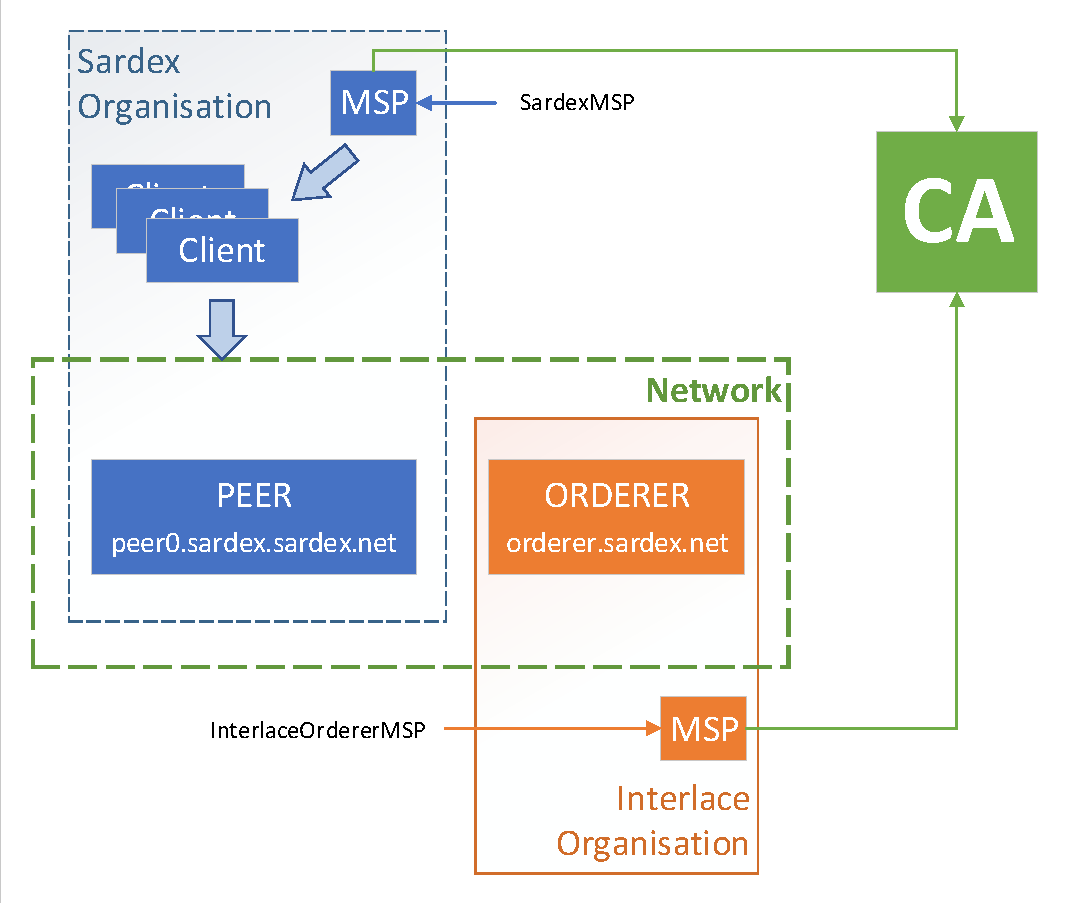
\includegraphics[width=0.7\textwidth, clip, trim=1mm 1mm 1mm 1mm]{Figures/basic-network}
  \caption{\bf\small Network structure implemented by the Prototype}
  \label{fig:prototype-net}
\end{figure}

The single \textbf{orderer} node in Figure \ref{fig:prototype-net} is responsible for atomic broadcasts, orders/batches transactions, and also signs each batch (block) to create unique and well-defined chains. The membership provider of the orderer uses a central and pre-configured certification authority \textbf{CA}.

This network configures and starts one \textbf{peer}. This peer can be called the core of the environment because its main task is to handle the so-called \textit{smart logic} (chaincode). More specifically, peers maintain the ledger by first endorsing a transaction (e.g.\ credit and debit transfers in the case of INTERLACE), which they do by simulating it.\footnote{This is the execution step in the Execute-Order-Validate Hyperledger architecture \cite{AndroulakiEtAl2018}} Then, in an intermediate step it is validated by the orderer and finally the peers commit it to their local ledger.

A very simple network is defined and described by the above scenario, which can be set up following the instructions of Section \ref{sec:prototype}. Certainly, this scenario needs to be extended to a real-world environment, a few hints and considerations for which will be given in Figure \ref{fig:prototype-net-ext} and explained in Section \ref{sec:future-scene}.

\subsection{Network Configuration Files}
\label{sec:net-conf-files}

There are three main configuration files providing a basic foundation for generating a preconfigured network. Those files are used to create the corresponding certificates as well as configuration files to spin up virtualised containers. Thus, the following three yaml files are an example of how to create a particular net as described in the previous section where the INTERLACE network was shown:

\begin{enumerate}
	\item crypto-config.yaml
	\item configfx.yaml
	\item docker-compose.yaml
\end{enumerate}

\textbf{crypto-config.yaml}

The \textit{crypto-config.yaml} contains the network topology and therefore defines its basic structure. With the configuration file it is possible to use a tool called \textit{cryptogen} which takes crypto-config.yaml as input to generate the cryptographic material necessary to run the blockchain. More specifically, \textit{cryptogen} generates the keys for both the organisations and the components that belong to those organisations.

Listing \ref{lst:cryConOrderers} shows a part of crypto-config.ymal that defines one or more orderers. The yaml definition of the network peers is depicted in Listing \ref{lst:cryConPeers}.

\begin{center}
\begin{minipage}{0.8\textwidth}
\small
\begin{lstlisting}[language=yaml,firstnumber=1,caption={\bf\small crypto-config.yaml excerpt -- Orderer(s) definition},captionpos=b,label=lst:cryConOrderers]
OrdererOrgs:
  # -----------------------------------------------------------------
  # Orderer
  # -----------------------------------------------------------------
  - Name: InterlaceOrderer
    Domain: sardex.net
    # ---------------------------------------------------------------
    # "Specs" - See PeerOrgs below for complete description
    # ---------------------------------------------------------------
    Specs:
  	  - Hostname: orderer
\end{lstlisting}
\end{minipage}
\end{center}

Listing \ref{lst:cryConOrderers} shows that in the case of INTERLACE only one orderer is specified in line 5, with the name \textit{InterlaceOrderer}. The network domain \textit{sardex.net} is defined with the \textit{Domain} key. Thus, together with the \textit{Hostname} definition in line 11, the INTERLACE orderer can be reached using \textit{orderer.sardex.net}.

Peers can be defined for the various organisations. For example, Listing \ref{lst:cryConPeers} shows the definitions specific to the INTERLACE project. The first and only organisation for now is \textit{Sardex} in the \textit{sardex.net} domain. Similarly, Sardex gets the \textit{Domain}-name \textit{sardex.sardex.net}. Taking a look at the hierarchy one level down, peers will receive domain names like peer0.sardex.sardex.net or peer1.sardex.sardex.net. As the template \textit{Count}-key only defines a value of \textit{1}, there will only be one peer with sub-domain name \textit{peer0}.

As mentioned above, user management is handled on a very small scale. Thus, when setting the user count to 0 in line 18 no users in addition to the administrator are defined.

\begin{center}
\begin{minipage}{0.8\textwidth}
\small
\begin{lstlisting}[language=yaml,firstnumber=1,caption={\bf\small crypto-config.yaml excerpt - Peer(s) definition}, captionpos=b,label=lst:cryConPeers]
PeerOrgs:
  # -----------------------------------------------------------------
  # Org1
  # -----------------------------------------------------------------
  - Name: Sardex
    Domain: sardex.sardex.net
    EnableNodeOUs: true
    # Peer nodes and if applicable host name templates
    # for the newly created peers
    Template:
      Count: 1
    # -----------------------------------------------------------------
    # "Users"
    # -----------------------------------------------------------------
    # Count: The number of user accounts _in addition_ to Admin
    # -----------------------------------------------------------------
    Users:
      Count: 0
\end{lstlisting}
\end{minipage}
\end{center}

For more details on how to configure the network to a greater depth, kindly consult the official Hyperledger Fabric documentation,\footnote{\url{https://hyperledger-fabric.readthedocs.io}} which is a valuable source and should be studied in detail in order to build Fabric-based networks.

In addition to the original Fabric documentation a reference guide called "Hands-On Blockchain with Hyperledger" \cite{HandsOnBlockchainHyperledger2018} was used to build this network.

\textbf{configtx.yaml}

The second configuration file is named \textit{configtx.yaml} and contains different but also some redundant configuration bits for the blockchain network. Another tool called \textit{configtxgen} picks up configtx.yaml and uses it to create configuration artefacts, thereby setting up a basic structure utilized by the actual blockchain network. These artefacts are:

\begin{itemize}
	\item orderer \textit{genesis block}
	\item channel \textit{configuration transaction}
	\item an \textit{anchor peer transaction} for each peer organisation
\end{itemize}

As stated in the Fabric documentation,\footnote{\url{https://hyperledger-fabric.readthedocs.io/en/release-1.3/build_network.html}}
\begin{quote}
\small
The orderer block is the Genesis Block for the ordering service, and the channel configuration transaction file is broadcast to the orderer at Channel creation time. The anchor peer transactions, as the name might suggest, specify each Organisation's Anchor Peer on this channel.
\end{quote}

The core configuration excerpt can be seen in Listing \ref{lst:configTxProfiles}. First, it defines an orderer genesis block called \textit{InterlaceOrdererGenesis} containing one orderer handled by organization \textit{Interlace} together with some capabilities (not discussed here) as well as a consortium using the network.

Second, it sets up a channel \textit{InterlaceChannel} which is connected to a consortium named \textit{InterlaceConsoritum}. This channel is used for credit and debit operations where currently only one organisation is defined: namely, \textit{Sardex}.

Third, as mentioned initially, anchor peers are recorded into the ledger. This is done by submitting a transaction to the ledger which contains the main anchor peers. Anchor peers may be defined for an organization using the config-property \textit{AnchorPeers}. The project defines a host called \textit{"peer0.sardex.sardex.net"} that provides services at port \textit{"7051"}, consistently with the crypto-config.yaml file. The host information is written into that initial transaction.

\begin{center}
\vspace{-.3cm}
\begin{minipage}{0.8\textwidth}
\small
\begin{lstlisting}[language=yaml,firstnumber=1,caption={\bf\small configtx.yaml excerpt -- Profiles definition}, captionpos=b,label=lst:configTxProfiles]
Profiles:
    InterlaceOrdererGenesis:
        Capabilities:
            <<: *ChannelCapabilities
        Orderer:
            <<: *OrdererDefaults
            Organizations:
                - *Interlace
            Capabilities:
                <<: *OrdererCapabilities
        Consortiums:
            InterlaceConsortium:
                Organizations:
                    - *Sardex
    InterlaceChannel:
        Consortium: InterlaceConsortium
        Application:
            <<: *ApplicationDefaults
            Organizations:
                - *Sardex
            Capabilities:
                <<: *ApplicationCapabilities
\end{lstlisting}
\end{minipage}
\vspace{-.3cm}
\end{center}

\textbf{docker-compose.yaml}

Docker and Docker Compose are the core technologies used to start containerized services which finally start the actual blockchain and its components. Hyperledger Fabric developer offer images which are ready to be started right away when provided with the correct configuration locations.

The compose file defines four container images. In Listing \ref{lst:composeImages} a shortened compose yaml-file shows the services (or images) started when \textit{docker-compose up} is called. One for the certification authority (line 2), one for the orderer (line 4), one for the peer (line 6), and also an additional container (line 8) the peer is storing data to. That additional container is a NoSQL database called CouchDB. 

\begin{center}
\begin{minipage}{0.8\textwidth}
\small
\begin{lstlisting}[language=yaml,firstnumber=1,caption={\bf\small docker-compose.yaml excerpt}, captionpos=b,label=lst:composeImages]
services:
  ca.sardex.sardex.net:
    [...]
  orderer.sardex.net:
    [...]
  peer0.sardex.sardex.net:
    [...]
  couchdb:
    [...]
\end{lstlisting}
\end{minipage}
\end{center}

Also docker-Composer creates a virtual network environment where the service containers defined here can communicate between themselves using the particular domain names used in this configuration file.

Each of the services starts its respective application, which handles the allotted requests. The certification authority (CA) is started by calling \textit{fabric-ca-server}, the orderer executes the eponymous command \textit{orderer}, the only peer (peer0) runs \textit{peer node start}, and the CouchDB image "couchdb" is started without specifying an additional command because the start-up process is handled by the container image itself.   

The CA might be replaced for a real-world production system by a different authority supporting ECDSA certificates. Fabric only supplies this implementation to get a network quickly up and running.

\textbf{Cryptographic Material}

Except for CouchDB, all other services need to be configured with the network structure as well as the appropriate public-private key infrastructure. In the \textit{chain} directory another folder called \textit{network} can be found. This folder contains templates of configtx.ymal as well as crypto-config.yaml. 

These template are, as mentioned, for generating the genesis block as well as the keys needed for the corresponing service. We have scripted the generation: it can be performed by calling \textit{build.sh}, which is also located in the same directory as the yaml-files. The results of running the build script are
\begin{itemize}
	\item interlace-channel.tx
	\item interlace-genesis.block
	\item crypto-config\ directory
\end{itemize}
These generated files as well as the directory are finally shared using docker volumes\footnote{\url{https://docs.docker.com/storage/volumes/}} for the respective services. A detailed description of how to configure the services can be found in the online documentation of Fabric\footnote{\url{https://hyperledger-fabric.readthedocs.io}} but also in \cite{HandsOnBlockchainHyperledger2018}.

%\subsection{cto-model}
%\label{sec:cto-model}

%The CTO-model is specific to Hyperledger Composer framework and offers a possibility to set-up a ground model which is imposed onto the chaincode implementation as well as on the blockchain residing on the peers. 

%The model created for INTERLACE project has 2 main \textit{transactions}, that are \textit{CreditTransfer} and \textit{DebitTransfer} and inherited by \textit{Transfer}. \textit{DebitTansfer} actually also needs a second transaction named \textit{DebitTransferAcknowledge} to be performed, thus it may be counted as a main transaction as well. Two other transactions supporting the functionality of the network are \textit{InitBlockchain} and \textit{CleanupPendingTransfer}.

%Transfers are handling \textit{assets}, which means creating and updating them. When the main transfers are executed they are changing \textit{Account}-assets, namely, \textit{SysAccount} and \textit{MemberAccount} which are inheriting from it. \textit{DebitTransfer} also needs \textit{PendingTransfer}-asset for creating transfers which haven't yet been confirmed. \textit{DeltaDebt} collects all transfers with the negative amount portion to log when the debt has to be paid back.

%\begin{figure}[htbp]
%  \centering
%  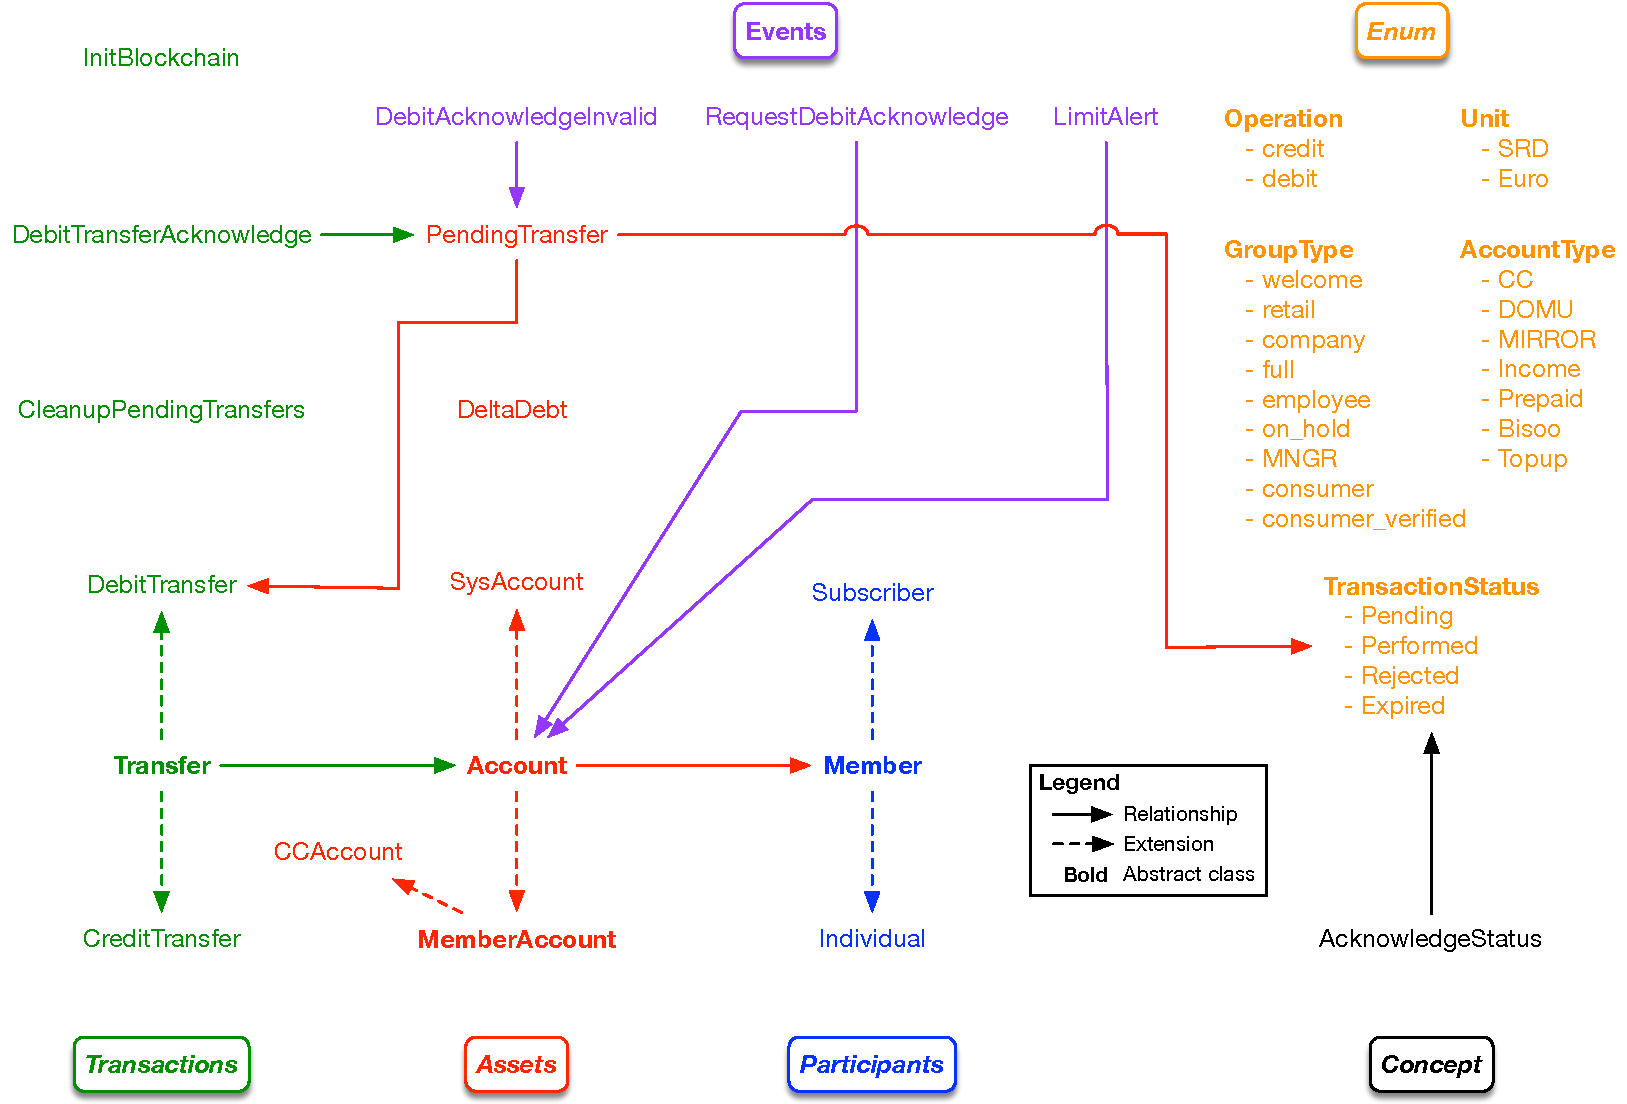
\includegraphics[width=1.0\textwidth]{Figures/cto-model}
%  \caption{\bf\small CTO Model Structure used by Hyperledger Composer}
%  \label{fig:DCN-cto}
%\end{figure}

%In order to perform credit or debit operations a \textit{participant} need to be registered. For the prototype they are quite reduced like the assets, however, there two participants derived from \textit{Member} called \textit{Subscriber} and \textit{Individual}. Those members may own an account asset which can be used then to transfer money from one account to another one.

%On several occasions event are emitted which may be consumed by an application or a user to react to specific issues happened during a transaction. There are many different events interesting for a user but for the moment there are three implemented. One is for a forecast of a possible limit violation named \textit{LimitViolation}, \textit{RequestDebitAcknowledge} asks a user to give an acknowledgement to a pending transaction and last \textit{DebitAcknowledgeInvalid} informs that the acknowledgement for a pending transaction got denied or has been invalid.

%Finally there are couple of \textit{enum} types giving states names like for operations and units as well as account and group types.

%A detailed explanation of the model language can be found the official Hyperledger Composer documentation\footnote{\url{https://hyperledger.github.io/composer/latest/reference/cto_language.html}}

\section{Prototype}
\label{sec:prototype}

The prototype is a blockchain realisation of INTERLACE, can be found on GitHub\footnote{\url{https://github.com/InterlaceProject/InterlaceBlockchain}} and is based on the specifications created in deliverable D3.1 \cite{INTERLACE_D31} along with the ASIM specification of the requirements.

First, it is necessary to install the prerequisites which are available for Linux and Mac OS. Currently these are the recommended operating systems. However, with additional effort it might be possible to run the INTERLACE blockchain on Windows directly. To support Windows users a virtual machine set-up is also available.

Additionally, it is also important to set up a development environment described in the Composer GitHub repository. Even if development is not planned and setting up a complete environment not necessary, it is still advisable to install and start Composer Playground. Playground enables someone to connect, alter, and test the INTERLACE payment network. Nevertheless, Playground is not required and it might be possible to use composer-cli or other methods to utilise the network.

\subsection{Install}
\label{subsec:install}
This part of the documents talks about how to set up and run the business network on your machine. However, before it is actually possible to begin it is necessary to install the pre-requisites which are listed at the Hyperledger Composer documentation.\footnote{\url{https://hyperledger.github.io/composer/latest/installing/installing-prereqs.html}} The website also offers a download where a script for installing all the requirements for a machine is provided.

Nevertheless, for Windows users these scripts won't help because for now most of the packages are not yet prepared (as of this writing) for a Windows operating systems. We have prepared a virtual machine also for this user group, which also installs all the necessary frameworks and software tools during provisioning. This virtual machine is controlled by vagrant\footnote{\url{https://www.vagrantup.com/}} and uses hyper-v or virtual box as hypervisor (two different branches). This VM configuration is published at GitHub\footnote{\url{https://github.com/hirsche/hyperledger}}.

\textbf{Environment Start-Up}

Once the Hyperledger environment is installed, the next step is to start the INTERLACE environment. To make communications uniform the blockchain is configured to publish all services under the host name "interlace.chain". To facilitate Windows users, in the suggested vagrant set-up the new hostname is added to your host-file at start-up time using the vagrant-hostmanager plug-in. Thus there is no need to configure the name manually.

\textbf{Configure Hostnames}

For non-vagrant users it is important before executing the local set-up to add a host name entry for "interlace.chain". Usually this entry will point to IP 127.0.0.1 (localhost). On a production system or if it was chosen to start the Hyperledger Composer services on a public interface, the IP needs to be fixed accordingly. Here is a list of host file locations according to different operating systems types:

\begin{itemize}
	\item Mac OS: /private/etc/hosts
    \item Linux: /etc/hosts
    \item Windows: C:\textbackslash Windows\textbackslash System32\textbackslash drivers\textbackslash etc\textbackslash hosts
\end{itemize}

The format may vary a little but usually a new host with its hostname is defined using its IP and the desired host name as

\begin{lstlisting}
	127.0.0.1        interlace.chain
\end{lstlisting}
Depending on the operating system, it might be also necessary to update and restart the corresponding services (e.g. MacOS).

\textbf{Run the Fabric blockchain (the first time)}

At this stage, the main configurations have been performed and Hyperledger Fabric can be started, which acts as a base for Hyperledger Composer. To continue, if not yet done the GitHub repository\footnote{\url{https://github.com/InterlaceProject/InterlaceBlockchain}} needs to be downloaded by using the git visioning system by calling:

\begin{lstlisting}[language=bash]
	git clone https://github.com/InterlaceProject/InterlaceBlockchain.git
\end{lstlisting}

In the directory "InterlaceBlockchain" that is created the business network implementation, including a web application, can be found. The next listing shows the bash script that downloads several Fabric docker containers and finally starts them using docker-composer:\footnote{\url{https://docs.docker.com/compose/}}

\begin{lstlisting}[language=bash]
	cd fabric
	./downloadFabric.sh # updates images - only the first time necessary
	./startFabric.sh # start up docker environment using docker-compose
\end{lstlisting}


%\textcolor{red}{Paolo: to here (2018-11-20)}


\textbf{Initialize Interlace-Chain}

Finally, after Fabric has been started the next step is to initialize the blockchain with

\begin{lstlisting}[language=bash]
	cd chain
	./initNetwork.sh # use Hyperledger Composer to create a business network and deploy it
\end{lstlisting}

\textbf{./initNetwork.sh} will copy all models and script to the network peers to make them accessible in the Hyperledger blockchain. The last step in the script starts the business network.

It may be more convenient to access the network and test CreditTransfer or DebitTransfer transactions using Playground. \textbf{data.json} should act as a helper to initialise the network by hand, but it is recommended to update the JavaScript function \textit{initBlockchain(transfer)} in \textit{./chain/lib/init.js}. That chaincode part is executed when transaction InitBlockchain is submitted. Be careful to run \textbf{InitBlockchain} only once otherwise errors or duplicate entries might happen resulting in an inconsistent chain.

\textbf{Network updates after chaincode changes}

After changes to the acl, cto, queries, the libraries, or other parts of the core chaincode application, the network needs to be updated. This can be achieved by executing

\begin{lstlisting}[language=bash]
	cd chain
	./updateNetwork.sh
\end{lstlisting}

This script reads the current version number of the \textit{package.json} file, increments it by one, and creates a new bna package. If the scripts are correct and the bna-package can be created it is deployed to the peers and the network is updated to a new, higher network version which will utilize the new bna package.

\textbf{Shutting down}

Sometimes it is useful to throw away everything and restart from scratch. To tear down Fabric and remove card left-overs execute:

\begin{lstlisting}[language=bash]
	cd fabric
	./teardownFabric.sh
	./deletePlaygroundCards.sh
\end{lstlisting}

\textbf{Start a REST server}

Once the network is running (no Playground needed) it is also possible to start an HTTP Server which allows to interact with the network over REST. The script

\begin{lstlisting}[language=bash]
	cd chain
	./startRestServer.sh
\end{lstlisting}

starts the server and provides GUI access to the RESTful interface by opening

\url{http://interlace.chain:3000/explorer}

in a browser. When accessing the REST interface from an external application, it may be reached over

\url{http://interlace.chain:3000/}

If the host interlace.chain has not been set up and all the services are running locally without a VM, it might be also possible to use localhost instead of interlace.chain as host name. Nevertheless, it is highly recommended to use "interalce.chain" because everything has been tested using that particular host name.

\subsection{Working with the environment}

Next, a closer look is taken on how the environment might be facilitated using different approaches. It is possible to connect to the chain using composer-cli, taking advantage of Composer Playground (the graphical interface) or using the simple web front-end created for the project.

\textbf{Start and test network with Playground}

If you've decided to install and use Composer Playground it can be started using this command

\begin{lstlisting}[language=bash]
	composer-playground
\end{lstlisting}

The standard configuration opens a browser connecting to Playground at localhost with port 8080. If you are running Playground in a separate virtual environment like e.g.\ in a docker container, it may be necessary to start the browser manually, determine the VM/Containers IPs, and fill in the address manually in the URL field.

\textbf{The Admin Cards}

Composer Playground helps by providing a basic web interface to interact with the Hyperledger Fabric blockchain, on top of which Hyperledger Composer acts as an additional wrapper. Composer creates cards in order to connect to the blockchain. These cards can be created over the Playground web interface or over the command line interface. For INTERLACE these cards are created by \textit{initNetwork.sh}, which is explained in Section \ref{sec:prototype}. When these scripts are executed, and no error messages are issued, two cards should have been created and should become visible when opening Hyperledger Playground. This is illustrated in Figure \ref{fig:admin-cards}.

\begin{figure}[htbp]
  \centering
  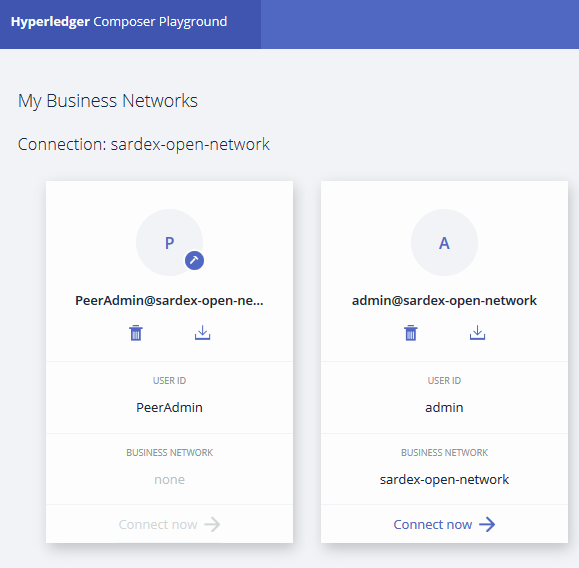
\includegraphics[width=0.5\textwidth]{Figures/admin-cards}
  \caption{\bf\small Admin Cards in Hyperledger Playground}
  \label{fig:admin-cards}
\end{figure}

These cards provide all the information needed to connect to the INTERLACE blockchain business network. In particular, in the present case two cards are installed:

\begin{itemize}
	\item Peer Admin Card (PeerAdmin@sardex-open-network)
	\item Business Network Card (admin@sardex-open-network)
\end{itemize}

\textit{Peer Admin Cards} are cards (as the name suggests) used to interact with the peers. Users connecting over that card receive the permissions to manage chaincode deployments or changes on the peers. Thus they are a crucial part of every network.

Access to Interlace/Sardex Business Network is granted to another user through the provision of a \textit{Business Network Card} which is called \textit{admin@sardex-open-network}.

For INTERLACE we currently only have one user in place, the admin user. However, if the network gets deployed it will become necessary to grant access to other users, which can be done by creating an additional Business Network Card for each new user. Be aware that for each new user a participant needs to be registered first in order to link it with a new network card. 

\textbf{Edit Network}

Figure \ref{fig:edit-network} illustrates how a particular business network may be edited over Playground directly. For INTERLACE this means that you can e.g.\ quickly try out some changes on the JavaScript files and see if the changes are deployable by pressing the "Deploy changes" button. However, most developers might prefer using a common IDE,\footnote{\url{https://en.wikipedia.org/wiki/Integrated_development_environment}} which offers far better assistance during development, and use the scripts \textit{initNetwork.sh} and \textit{updateNetwork.sh} provided.

\begin{figure}[htbp]
  \centering
  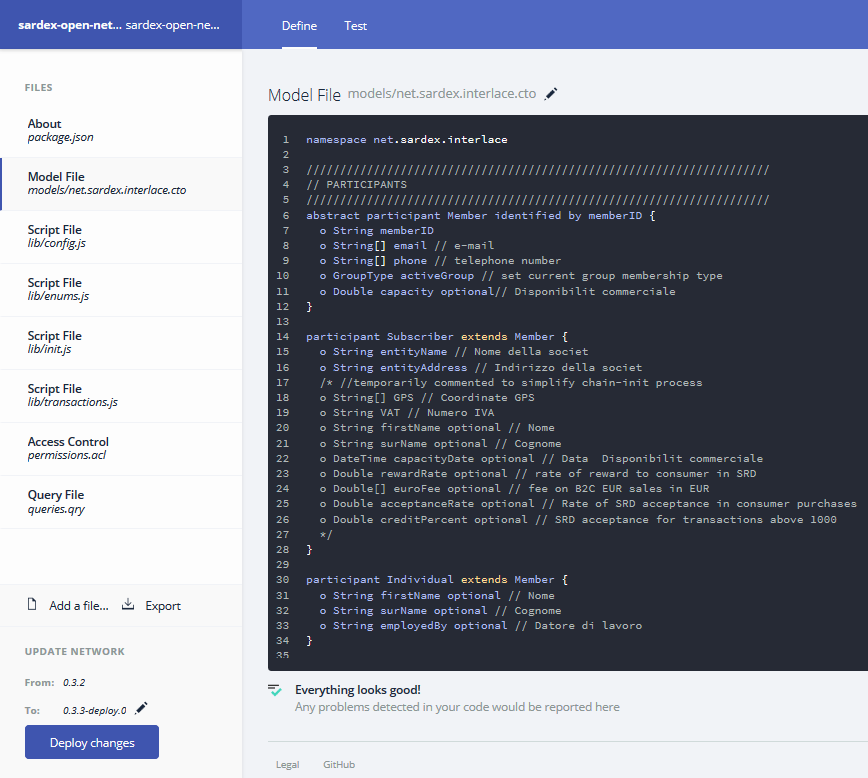
\includegraphics[width=0.6\textwidth]{Figures/edit-network}
  \caption{\bf\small Edit a network in Hyperledger Playground}
  \label{fig:edit-network}
\end{figure}

\textbf{Test Network}

The INTERLACE blockchain might be also tested directly with Playground web interface instead of using the Composer cli tools or launching the additional web application provided. Figure \ref{fig:test-network} shows the Playground test environment that comes with Playground and is started by pressing "Test" in the menu bar.

On the left bar of that view you are provided with a list of the INTERLACE participants, assets, as well as entry call "All Transactions". As the menu names might suggest, when clicking on them a list of those items which have been created on the chain is displayed. E.g., this view in \ref{fig:test-network} lists all \textit{Individuals} taking part in the Interlace-Test network. As shown in the main area of the screenshot, two "Individual" participants have been registered. One member with ID "m1" and one with ID "m2".

In addition, it is possible here to add and change entries for participants and assets you might change for customised tests.

Finally, the "All Transactions" menu entry guides to a list of all transactions executed on the INTERLACE chain. This list contains of course not just the transactions somebody has submitted but also entries like e.g.\ "AddParticipant" or "IssueIdentity". Thus, all changes to the blockchain are recorded and can be found here.

\begin{figure}[htbp]
  \centering
  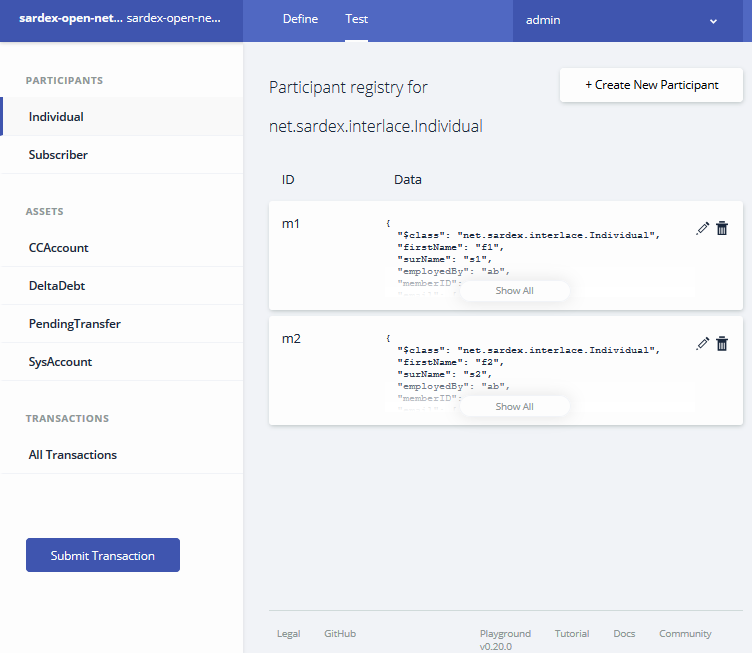
\includegraphics[width=0.7\textwidth]{Figures/test-network}
  \caption{\bf\small Test a network in Hyperledger Playground}
  \label{fig:test-network}
\end{figure}

\textbf{Submit a transaction}

Figure \ref{fig:submit-credit-transfer} shows a submission dialog, which opens when the "Submit Transaction" button in screenshot \ref{fig:test-network} is pressed. This dialog gives the possibility to select one of all possible transactions executable on the INTERLACE network. In this dialog a \textit{CreditTransfer} has been selected.

In the black text-box the properties of that transactions can be provided as a JSON-String. The interface provides default transaction-specific values.

\begin{figure}[htbp]
  \centering
  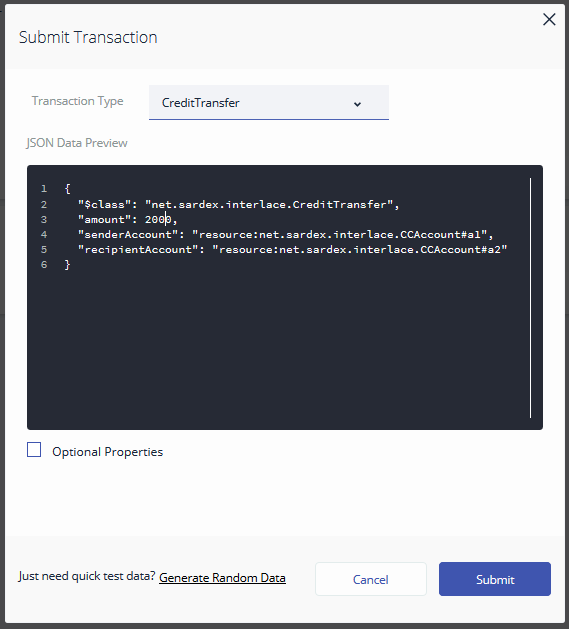
\includegraphics[width=0.5\textwidth]{Figures/submit-credit-transfer}
  \caption{\bf\small Submit a (credit) transfer in Hyperledger Playground}
  \label{fig:submit-credit-transfer}
\end{figure}

Once all the necessary properties have been provided, pressing "Submit" tries to commit the transaction to the blockchain. If an error is encountered, it is shown in red font attached to the same dialog. When everything goes as planned the transaction is endorsed, ordered, and committed to the peers. The execution results will finally show up in the JSON records used for the assets and participants as well as in the transaction log of the chain.

Details on how to configure and initialize INTERLACE transactions are covered in Section \ref{subsec:initblockchain} which discusses the technical details.

\textbf{Run Transactions with composer-cli}

Initialise network transaction:

\begin{lstlisting}[language=bash]
	composer transaction submit -c admin@sardex-open-network -d  '{ "$class": "net.sardex.interlace.InitBlockchain" }'
\end{lstlisting}

The InitBlockchain transaction sets up some basic accounts as well as demo members that can issue simple transactions right away.

Submit a credit transfer from account a1 to a2 with amount of 800 SRD:

\begin{lstlisting}[language=bash]
	composer transaction submit -c admin@sardex-open-network -d  '{ "$class": "net.sardex.interlace.CreditTransfer", "amount": 800, "fromAccount": "resource:net.sardex.interlace.CCAccount#a1", "toAccount": "resource:net.sardex.interlace.CCAccount#a2" }'
\end{lstlisting}

Submit a debit transfer from account a1 to a2 with amount of 200 SRD:

\begin{lstlisting}[language=bash]
	composer transaction submit -c admin@sardex-open-network -d  '{ "$class": "net.sardex.interlace.DebitTransfer", "amount": 200, "fromAccount": "resource:net.sardex.interlace.CCAccount#a1", "toAccount": "resource:net.sardex.interlace.CCAccount#a2" }'
\end{lstlisting}

A successful debit transfer creates a PendingTransfer entry with status Pending containing an OTP (one-time password). This OTP can be used by the debitor to confirm the transaction. Thus, in the next example "995317396" is used to call a transaction DebitTransferAcknowledge to acknowledge the debit transfer:

\begin{lstlisting}[language=bash]
	composer transaction submit -c admin@sardex-open-network -d  '{ "$class": "net.sardex.interlace.DebitTransferAcknowledge", "transfer": "resource:net.sardex.interlace.PendingTransfer#995317396" }'
\end{lstlisting}

\textbf{The web front-end}

The web front-end currently is a simple website generated by a Yeoman generator provided by the Composer community. The web application can be found in the web app directory.

In order to get the web application to run properly it is necessary to start up the whole network and start the REST server as described in the previous steps.

The web app is based on AngularJS and needs various node.js packages downloaded and installed, which is achieved by calling

\begin{lstlisting}[language=bash]
	cd webapp
	npm install
\end{lstlisting}

After that a development server can be started by calling

\begin{lstlisting}[language=bash]
	cd webapp
	npm start
\end{lstlisting}

npm will start a web server at port 4200. If you work locally it also tries to open a browser which shows the web application. Otherwise one needs to start a browser manually and enter the URL. This is the URL where the server can be reached:

\url{http://interlace.chain:4200}

The webpage is based on AngularJS and communicates over REST with our previously started REST server, enabling asynchronous AJAX-request.

\section{The Chaincode}
\label{sec:chaincode}

This section describes the core business logic, which is found in the \textit{chain} directory. The shell scripts ending with \textit{.sh} were discussed in Section \ref{sec:prototype}, except for \textit{startRestServer.sh} which is handled in the technical details Section \ref{sec:rest-server}. This section focuses on the chaincode implementation which is stored in the directory \textit{lib} illustrated in Figure \ref{fig:chain-structure}.

\begin{figure}[htbp]
\centering
\begin{minipage}{5cm}
\dirtree{%
.1 chain.
	.2 \textbf{lib/}.
		.3 config.js.
		.3 enums.js.
		.3 init.js.
		.3 transactions.js.
	.2 \textbf{models/}.
	.2 \textbf{network/}.
	.2 connection.json.
	.2 data.json.
	.2 \textcolor{green}{initNetwork.sh}.
	.2 package-lock.json.
	.2 package.json.
	.2 permissions.acl.
	.2 queries.qry.
	.2 \textcolor{green}{updateNetwork.sh}.
	.2 \textcolor{green}{startRestServer.sh}.
}
\end{minipage}
\caption{\bf\small Chaincode Directory Structure}
\label{fig:chain-structure}
\end{figure}


In the lib directory, \textit{config.js} contains the main configurations including things like time-outs, quick-transfer amounts, and transfer types and account type mappings, which are done in the form of a JSON object. Unfortunately, Composer doesn't offer static access to enumeration constants. All enumeration values of a type need to be addressed by a string value. This approach is quite dangerous and gives potentially space for a lot of common errors. INTERLACE tries to solve this issue by setting up an object with "frozen"\footnote{\url{https://developer.mozilla.org/en/docs/Web/JavaScript/Reference/Global_Objects/Object/freeze}} attributes.

In Listing \ref{lst:enumMap} a JavaScript mapping of the cto model enum type \textit{Unit} in \ref{lst:enumCTO} is illustrated.

\begin{center}
\begin{minipage}{0.8\textwidth}
\small
\begin{lstlisting}[language=javascript,firstnumber=1,caption={\bf\small JavaScript enumeration mapping}, captionpos=b,label=lst:enumMap]
var Unit = Object.freeze({
  'Euro': 'Euro',
  'SRD': 'SRD'
});
\end{lstlisting}
\end{minipage}
\end{center}

Using this way of enum-mapping, a proper development environment suggests and auto-completes the possible values of an e.g.\ Unit when the user works with it. Instead, there is the possibility, as mentioned, to directly work with string values. But writing \textit{Unit.Euro} instead of \textit{"Euro"} ensures during development when sources are linted\footnote{\url{https://en.wikipedia.org/wiki/Lint_\%28software\%29}} that the correct enumeration names have been applied.

\begin{center}
\begin{minipage}{0.8\textwidth}
\small
\begin{lstlisting}[language=cto,firstnumber=1,caption={\bf\small enum in CTO-model}, captionpos=b,label=lst:enumCTO]
enum Unit {
  o Euro
  o SRD
}
\end{lstlisting}
\end{minipage}
\end{center}

\subsection{Linking Transactions}
\label{sec:link transactions}

There are two JavaScript files which contain the available transactions of the network: \textit{init.js} and \textit{transactions.js}. Before going into the details of what these files contain, we give a simple example of how transactions of the CTO model are mapped to a JavaScript function. Listing \ref{lst:linkTransaction} gives a short example of the syntax through which \textit{CreditTransfer} transactions are linked to a JavaScript function with the same name.

\begin{center}
\begin{minipage}{0.8\textwidth}
\small
\begin{lstlisting}[language=javascript,firstnumber=1,caption={\bf\small Connection of JavaScript function CreditTransfer to CTO-model transaction type}, captionpos=b,label=lst:linkTransaction]
/**
 * CreditTransfer transaction
 * @param {net.sardex.interlace.CreditTransfer} transfer
 * @transaction
 */
async function CreditTransfer(transfer) { [...] }
\end{lstlisting}
\end{minipage}
\end{center}

In this example the JavaScript name of the function is not important. Rather, what matters is the notation \textit{@transaction}, as well as the definition of the parameter(s) of the function and of their type. More specifically, on line 3 the parameter \textit{transfer} is linked to the CTO model type \textit{net.sardex.interlace.CreditTransfer}. When a CreditTransfer is invoked, usually using a JSON string, this string is converted to a type in JavaScript that has the same properties as \textit{net.sardex.interlace.CreditTransfer} and that is provided as \textit{transfer} input parameter.

Then, during execution the \textit{transfer} input parameter may be used like any JavaScript object and contains all the information necessary to process that transaction request. In JS, it is important that the code be deterministic and that it evaluates to the same result on different peers.

\subsection{Init Blockchain}
\label{subsec:initblockchain}

The only transaction in \textit{init.js} should be executed only once, otherwise it will lead to an inconsistent blockchain if executed twice. The reason is that this initialisation script sets up a couple of participants with an account asset each to immediately test the blockchain. Thus, after the "InitBlockchain" transaction has been executed the chain contains at least two members and two accounts in order to move money around by applying credit and debit operations. Therefore, executing the initialisation multiple times will create a pair of participants each time, leading to a configuration that does not match other parts of the model.

Listing \ref{lst:initBlock} shows parts of the actual creation of an asset as well as of a participant. It uses \textit{getFactory()}, which is part of the Composer API to generate new instances of various types. The factory offers a function \textit{newResource} to actually create first an "Individual" from namespace \textit{net.sardex.interlace} and afterwards a "CCAccount" residing in the same namespace. The namespace is not visible in the script of Listing \ref{lst:initBlock} because it has been configured in the config.js file and applied to the config object.

Function \textit{newResource} uses namespace, type name, and identifier as parameters and, in the case of line 3, for example, gives back a JavaScript representation of "net.sardex.interlace.Individual". The same principle applies to line 8 when a CCAccount is created.

To write a new resource to the ledger a registry of the type super-category has to be acquired.

Given that the Individual is a participant, the \textit{getParticipantRegistry} function needs to be called in order to write it to the chain. For any asset like the CCAccount, it is necessary to call the \textit{getAssetRegistry} function to receive the right registry.

\begin{center}
\begin{minipage}{0.8\textwidth}
\small
\begin{lstlisting}[language=javascript,firstnumber=1,caption={\bf\small Chaincode adding a new resource in \textit{initBlockchain} function}, captionpos=b,label=lst:initBlock]
let factory = getFactory();

let m1 = factory.newResource(config.NS, 'Individual', 'm1');
m1.firstName='f1';
[...]

let a1 = factory.newResource(config.NS, 'CCAccount', 'a1');
[...]
a1.balance=1000;
a1.member=factory.newRelationship(config.NS, 'Individual', 'm1');
[...]

let partReg = await getParticipantRegistry(config.NS + '.Individual');
await partReg.addAll([m1]);

let accReg = await getAssetRegistry(config.NS + '.CCAccount');
await accReg.addAll([a1]);
\end{lstlisting}
\end{minipage}
\end{center}

Once the registries are available, they can be called as in lines 14 and 17 with the matching type-category, to finally ask to add a new entry to the chain. The Hyperledger Composer API also has  functions for reading, removing or update included. The documentation for the AssetRegistry\footnote{\url{https://hyperledger.github.io/composer/v0.19/api/runtime-assetregistry}} and for the \textit{ParticipantRegistry}\footnote{\url{https://hyperledger.github.io/composer/v0.19/api/runtime-participantregistry}} can be found in the Composer documentation.

\subsection{Main Payment Transactions}
\label{subsec:main-payment-transactions}
The current implementation comes with credit and debit transactions that work according to the specifications made in D2.1 \cite{INTERLACE_D21} and D3.1 \cite{INTERLACE_D31}, except for the requirement concerning the tracking of the debt position over time, \textit{DeltaDebt}, which can be found in D2.3 \cite{INTERLACE_D23}.

\textbf{CreditTransfer chaincode}

Let's now focus on the first of the two payment transactions: the credit transfer. Listing \ref{lst:js-credittransfer} shows the core of the JavaScript function without the additional function wrappers.

The code was written in a way that is supposed to be readable by people who may not be JavaScript experts. Nevertheless, the keyword \textit{await} might  need a brief explanation:\footnote{\url{https://developer.mozilla.org/en-US/docs/Web/JavaScript/Reference/Operators/await}} \textit{await} deals with asynchronous JavaScript function calls and (in simplified terms) just waits until the prefixed function completes its task. If \textit{await} were missing, an asynchronous JavaScript (like previewCheck) would be called and executed in the background and the execution of the current thread would continue immediately.

\begin{center}
\begin{minipage}{0.8\textwidth}
\small
\begin{lstlisting}[language=javascript,firstnumber=1,caption={\bf\small CreditTransfer JavaScript}, captionpos=b,label=lst:js-credittransfer]
//some basic checks
await checkAmountPlausible(transfer);

// preview check throws error in case of violation
await previewCheck(transfer);

// account limits checks throws error in case of violation
await accountLimitCheck(
  transfer.fromAccount,
  transfer.toAccount,
  transfer.amount);

// check account limits and emits event if violated
await checkAccountLimitsAlerts(transfer.fromAccount);

// perform the transfer
await moveMoney(transfer);
\end{lstlisting}
\end{minipage}
\end{center}

The \textit{transfer} object used in the listing is pre-filled by the chaincode API after a CreditTransfer is invoked. It is created from the parameters and values of the JSON object that is part of the submitted transaction and that follows the structure of the CTO model of type \textit{net.sardex.interlace.CreditTransfer}.

\textbf{DebitTransfer chaincode}

The debit operation, shown in Listing \ref{lst:js-debittransfer}, is a bit more complex compared to a basic credit operation. In that listing only the important part of the function is shown. The leading part calling \textit{checkAmountPlausible}, \textit{previewCheck}, and \textit{accountLimitCheck} is exactly the same as in CreditTransfer and, therefore, it was left out to increase readability.

One note for debit operations resulting from the specifications is that the owner of the fromAccount from the debit transfer is the debitor, who is also the buyer. Whereas the toAccount owner is regarded as the creditor who is selling something. Please see Figure 2.7 in D3.1 \cite{INTERLACE_D31} for the definition of fromAccount, toAccount, and related concepts.

Continuing further with the implementation, the core of the debit operation checks if an immediate transfer is possible (amount smaller than a predefined value) or if a confirmation of the other party is necessary. In case of an immediate transfer the money is moved the same way as in CreditTransfer by calling the \textit{moveMoney} function. If the transfer amount is above a threshold (currently 100 SRD), however, a confirmation needs to be obtained from the debitor who is in our case the owner of the fromAccount of the transfer.

\begin{center}
\begin{minipage}{0.8\textwidth}
\small
\begin{lstlisting}[language=javascript,firstnumber=1,caption={\bf\small DebitTransfer JavaScript}, captionpos=b,label=lst:js-debittransfer]
// check for immediate transfer possibility
if (transfer.amount <= config.debit.quick_transfer_amount) {
  // perform the transfer
  await moveMoney(transfer);

  // check account limits and emits event if violated
  await checkAccountLimitsAlerts(transfer.fromAccount);
} else { // requires confirmation
  // add the debit transfer to the pending queue
  let otp = await insertPendingTransfer(transfer);

  // create confirmation event RequestDebitAckReqAnswCompletion
  // which is including the OTP and the sender account (of debitor)
  [...]

  // emit the event
  emit(confirmReq);
}
\end{lstlisting}
\end{minipage}
\end{center}

If a confirmation is needed the transaction \textit{DebitTransfer} cannot move the amount from account A to account B instantaneously. To remember all values of that transaction they are stored inside asset \textit{PendingTransfer} which uses an OTP as identifier. The insertion done by Function \textit{insertPendingTransfer} returns a new OTP when successfully, creating a transfer which is awaiting confirmation.

In order to tell a user that there is a pending confirmation waiting \text{DebitTransfer} issues an event called \textit{RequestDebitAcknowledge} of namespace \textit{net.sardex.interlace} defined in the CTO model. When instantiated, the event obtains a reference to the just created \textit{PendingTransfer} which is done by using the \textit{factory} object (received by the composer API) and calling \textit{newRelationship} which utilizes the OTP references.

\textbf{DebitTransferAcknowledge chaincode}

Each entry in PendingTransfer is identified by an OTP in a way that a transfer can be unambiguously selected by providing an OTP. Currently the OTP is generated by hashing the transaction id of the debit transfer. However, if a debitor would like to confirm a transfer of which he was informed by the emitted event, he just needs to pass the OTP as property for the \textit{DebitTransferAcknowledge} transaction.

\textbf{Note:} For production systems this identification might include an additional key since for large numbers of PendingTransfers the OTP generated in this way might not be unique anymore.

Listing \ref{lst:js-ack} shows the main part of \textit{DebitTransferAcknowledge}, which is different from the other transactions. The variable \textit{ack} in the script is a transaction object provided to the function which contains the \textit{PendingTransfer} read into variable \textit{pT}. Then the code tries to verify the \textit{TransactionStatus}. If the transaction is in state \textit{Pending} it may proceed; in any other case an error is thrown and the transaction is discarded (!not! recorded into the ledger).

If the process is continued the timestamp of the transaction is checked against the \textit{expires} date property of the pending transfer. Consequently, if expired, the state is updated to \textit{"Expired"} and function \textit{DebitTransferAcknowledge} returns with the corresponding status \textit{AcknowledgeStatus}.

\begin{center}
\begin{minipage}{0.8\textwidth}
\small
\begin{lstlisting}[language=javascript,firstnumber=1,caption={\bf\small RequestDebitAcknowledge JavaScript excerpt}, captionpos=b,label=lst:js-ack]
[..]
//get pending transaction
let pT = ack.transfer;

// verify state of pending transfer
if (pT.state !== TransactionStatus.Pending) {
  throw new Error('Transfer is not in state "' +
    TransactionStatus.Pending + '" but in state "' + pT.state + '"');
}

// varify if pending transaction has been expired
if (ack.timestamp >= pT.expires) {
  //update state from Pending to Rejected
  await updatePendingTransaction(pT, TransactionStatus.Expired);

  //prepare return message
  rS.status = TransactionStatus.Expired;
  rS.description = 'OTP ' + pT.otp + ' is expired.';
  return rS; //TODO: raise event
}
[..]
\end{lstlisting}
\end{minipage}
\end{center}

In the later parts of the function, after all of the checks have been passed and the debit transaction can be performed, the execution steps are pretty much the same as in a CreditTransfer. The only difference is that in case of success or error the PendingTransfer asset of the transaction needs to be updated to Performed or Rejected, respectively. A function called \textit{updatePendingTransaction}, also used in line 14 of Listing \ref{lst:js-ack}, takes care of putting the asset PendingTransfer into the right state.

Additionally, in all cases in which \textit{updatePendingTransaction} has been applied, also a status object called \textit{AcknowledgeStatus} is created and returned by the function that contains the resulting status, along with an error message if something went wrong.

\textbf{moveMoney \& DeltaDebt}

Actual movement of an amount from one to an other account is performed by basic addition and subtraction applied to the balances of the respective accounts and, finally, by updating the account assets in the ledger by means of the registry provided by the Hyperledger Composer API.

Another important step, however, which is part of this money transfer and is shown in Listing \ref{lst:js-movemoney}, is an additional functionality which was specified in D2.3 \cite{INTERLACE_D23}. This logic collects all debts, thus, every transactions which are causing the balance to go negative or to increase (in absolute value) an already negative balance. These debts are collected because they are handled similarly to a loan. ALthough they don't incur interest or any additional fees, these debts have a due date of 12 months by when they need to be paid back. See the Appendix of \cite{INTERLACE_D23} for more details.

\begin{center}
\begin{minipage}{0.8\textwidth}
\small
\begin{lstlisting}[language=javascript,firstnumber=1,caption={\bf\small moveMoney JavaScript excerpt}, captionpos=b,label=lst:js-movemoney]
[..]
// check balance if DeltaDebt entry needs to be added
// !after amount has been substracted!
if (transfer.fromAccount.balance < 0) await createDeltaDebt(transfer);
// check balance if clearing an open DeltaDebt is necessary
// !before amount has been added!
if ((transfer.toAccount.balance - transfer.amount) < 0) {
  await clearDebt(transfer);
}
[..]
\end{lstlisting}
\end{minipage}
\end{center}

The creation of a debt handled by \textit{createDeltaDebt} is straightforward and just adds an entry to asset \textit{DeltaDebt} if a transaction has been detected which causes a negative balance or makes an already negative balance more negative. A new \textit{DeltaDebt} entry receives an original amount, a current amount, an owner id, and of course a due date by when it needs to be paid back.

If however a transaction adds money to the account owner's balance, say with a positive amount "Amount", former \textit{DeltaDebt} entries may be cleared, which is done by querying all debts with a still unpaid amount. This is illustrated in Listing \ref{lst:js-cleardebt}, where a rich query called \textit{selectDeltaDebt} is used to account for all of those unpaid debts. Details of this and other queries are discussed in subsection \ref{subsec:queries}.

\begin{center}
\begin{minipage}{0.8\textwidth}
\small
\begin{lstlisting}[language=javascript,firstnumber=1,caption={\bf\small clearDebt JavaScript excerpt}, captionpos=b,label=lst:js-cleardebt]
// query result sorted by "oldest" first
let openDelta =
  await query('selectDeltaDebt', {ID: (transfer.toAccount.member.memberID)});
\end{lstlisting}
\end{minipage}
\end{center}

All selected debts are iterated, starting with the oldest first. The available portion of Amount gets subtracted from the current \textit{DeltaDebt} asset. If Amount is bigger than the current debt being examined, the rest of Amount ($amount = amount - deptPos$) is used in the next iteration step towards the clearing of the next-oldest entry of \textit{DeltaDebt}. Thus, this loop continues either until Amount has been all used up or all debts have been paid back, which also means in the latter case that the balance goes back to having a zero or positive value.

\subsection{Additional Transactions}

There is an additional transaction important for maintenance issues. This transaction, called \textit{CleanupPendingTransfer}, is illustrated in Listing \ref{lst:js-cleanupPending} and takes care of handling old entries of asset \textit{PendingTransfer}.

In some cases pending transfers stay unconfirmed for ever because they e.g.\ were issued wrongly by a user, or were duplicates if a connection had been interrupted together with a lost emitted acknowledge-request event. In such cases, for legal and security reasons these transfers have to be set to \textit{Expired}.

\begin{center}
\begin{minipage}{0.8\textwidth}
\small
\begin{lstlisting}[language=javascript,firstnumber=1,caption={\bf\small clearDebt JavaScript excerpt}, captionpos=b,label=lst:js-cleanupPending]
let expiredPending =
  await query('selectExpiredPendingTransfers', {now: (transfer.timestamp)});
let aR = await getAssetRegistry(config.NS + '.PendingTransfer');

// change all states to expired
expiredPending.forEach(p => p.state = TransactionStatus.Expired);
await aR.updateAll(expiredPending);
\end{lstlisting}
\end{minipage}
\end{center}

First, the chaincode shown selects all expired entries with query \textit{selectExpiredPendingTransfers}. Then it iterates all of them applying the new state. Finally, all entries are updated using the \textit{AssetRegistry}.

As this is a maintenance transaction it should be executed only by an admin or a user with a specific maintenance role.

\subsection{Queries}
\label{subsec:queries}

Using Hyperledger Composer it is easily possible to read data written into the ledger. This can be done by using its bespoke query language by defining a file called \textit{queries.qry}. 

The Hyperledger Composer Query Language\footnote{\url{https://hyperledger.github.io/composer/v0.19/reference/query-language}} is used in INTERLACE to read information about \textit{PendingTransfer} as well as about \textit{DeltaDebt}. Although looking like SQL a very limited set of operators are possible to use. Nevertheless, for INTERLACE this limitations are not relevant because simple selection and filtering is sufficient which can be observed looking at listing \ref{lst:queries}.

The first query in the listing \textit{selectExpiredPendingTransfers} is used by transaction \textit{CleanupPendingTransfers} to find all transfers which are outdated and should be marked as \textit{Expired}. In detail the \textit{SELECT} keyword expects an asset defined in the CTO and will return all of the entries in the ledger filtered by the \textit{WHERE} condition.

\begin{center}
\begin{minipage}{0.8\textwidth}
\small
\begin{lstlisting}[language=sql,firstnumber=1,caption={\bf\small INTERLACE business network queries}, captionpos=b,label=lst:queries]
query selectExpiredPendingTransfers {
  description: "select all expired transfer which are still in state pending"
  statement:
      SELECT net.sardex.interlace.PendingTransfer
       WHERE ((expires <= _$now) AND (state == 'Pending'))
}
query selectDeltaDebt {
  description: "select all open debts"
  statement:
      SELECT net.sardex.interlace.DeltaDebt
       WHERE ((deptPos > 0) AND (debitorID == _$ID))
       ORDER BY [created ASC]
}
\end{lstlisting}
\end{minipage}
\end{center}

Here we filter against property \textit{expires} and state equals to 'Pending'. Parameters like \textit{\_\$now} may be supplied using a JSON like reference from JavaScript\footnote{\url{https://hyperledger.github.io/composer/v0.19/api/client-businessnetworkconnection\#buildquery}}.

In query \textit{selectDeltaDebt} all open debts for particular debitor (which is a member of the circuit) having id \textit{\_\$ID} are selected. Like parameter \textit{\_\$now}, parameter \textit{\_\$ID} needs to be set by the calling counterpart.

\subsection{Access Control Language File}

The INTERLACE prototype currently only has one user which is also the admin and user of the whole network - for no other users certificates have been issued.  This can be easily changed by adopting the acl-file of the implementation and binding certificates to participants.  However, to reduce complexity especially for people who work first with the demo implementation the set-up has been kept simple in this regards.

In listing \ref{lst:acl-permissions} you may find the INTERLACE Access Control Language file, permissons.acl, which grants access to any user with any operation available.  

\begin{center}
\begin{minipage}{0.8\textwidth}
\small
\begin{lstlisting}[language=json,firstnumber=1,caption={\bf\small access  control configuration for INTERLACE}, captionpos=b,label=lst:acl-permissions]
rule Default {
    description: "Allow all participants access to all resources"
    participant: "ANY"
    operation: ALL
    resource: "net.sardex.interlace.*"
    action: ALLOW
}

rule SystemACL {
  description:  "System ACL to permit all access"
  participant: "ANY"
  operation: ALL
  resource: "org.hyperledger.composer.system.**"
  action: ALLOW
}
\end{lstlisting}
\end{minipage}
\end{center}

Details on how to refine access can be found at the Hyperledger Composer documentation\footnote{\url{https://hyperledger.github.io/composer/v0.19/tutorials/acl-trading}}.

\subsection{Deployment}

The deployment of the chaincode application has to happen in several steps which are, as mentioned in section \ref{subsec:install}, handled by \textit{initNetwork.sh} or after consecutive changes with \textit{updateNetwork.sh}. Both scripts utilize the hyperledger composer-cli component.

The script \textit{initNetwork.sh} needs to

\begin{enumerate}
	\item create package.json if not existing
	\item packing all sources into a bna-file,
	\item create a network card for the \textit{ChannelAdmin} as well as the \textit{PeerAdmin} roles,
	\item import that card,
	\item install the new network,
	\item start the new network,
	\item and finally import the network admin card generated by the starting process.
\end{enumerate}

Basically, the script will provide a running business network together with composer cards which are connection profiles used to access the network.

During development the network usually needs to be deployed a couple of times to check and test the implementations. For that purpose \textit{updateNetwork.sh} has been created. It reduces these 7 steps necessary for initial install to just 4 handling an intermediate update. These steps are

\begin{enumerate}
	\item increasing the version of the business network implementation,
	\item re-packing the changed sources into a bna-file having a higher version tag,
	\item installing the new bna-file on the network,
	\item and at last upgrading the network to the new version.
\end{enumerate}

\section{Rest Server}
\label{sec:rest-server}

A REST server used for connections of client applications can be provided by the Hyperledger Composer Rest Server CLI-Tool\footnote{\url{https://hyperledger.github.io/composer/latest/reference/rest-server}}. The REST server is able to connect to the business network and provides access to all assets, transactions and queries available on the network.

For INTERLACE all the configurations necessary to run that server are gathered inside \textit{startRestServer.sh}. The exposed REST API is shown in figure \ref{fig:rest-swagger} and is build with Swagger tools\footnote{\url{https://swagger.io/}}.

\begin{figure}[htbp]
  \centering
  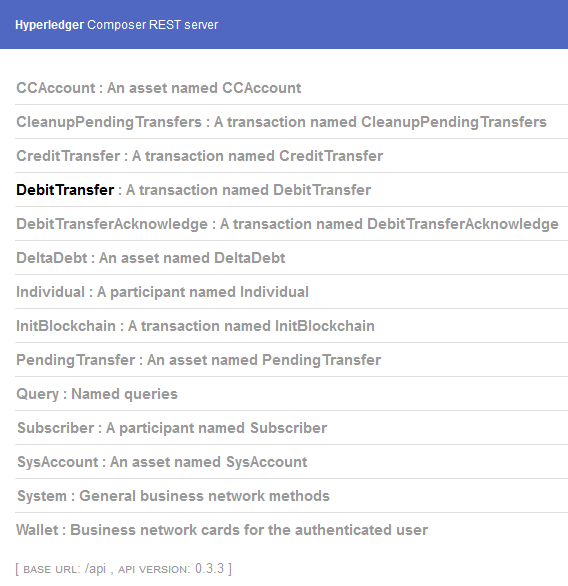
\includegraphics[width=0.7\textwidth]{Figures/rest-swagger}
  \caption{\bf\small REST GUI provided by composer-rest-server using Swagger}
  \label{fig:rest-swagger}
\end{figure}

\section{Web Application}
\label{sec:webapp}

In figure \ref{fig:webapp} an illustration of a web page generated for the INTERLACE business network implementation is shown. It has been created using generator-hyperledger-composer\footnote{\url{https://www.npmjs.com/package/generator-hyperledger-composer}} which is a yeoman\footnote{\url{http://yeoman.io/}} module.

\begin{figure}[htbp]
  \centering
  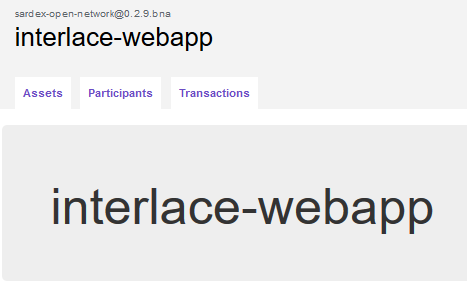
\includegraphics[width=0.8\textwidth]{Figures/webapp}
  \caption{\bf\small An AngularJS based web-application }
  \label{fig:webapp}
\end{figure}

From that web-application it is possible to list, add and edit assets and participants as well as submit transactions to the network. It is implemented in AngularJS\footnote{\url{https://angular.io/}} and connects to the REST server which is, as mentioned, also provided by the composer tool-suit.

Consequently, it is possible to manage assets like \textit{SysAccount}, \textit{CCAccount}, \textit{PendingTransfer}, \textit{DeltaDebt}. Participants like \textit{Subscriber} and \textit{Individual} are using these assets whereas transaction \textit{CreditTransfer}, \textit{DebitTransfer}, \textit{DebitTransferAcknowledge} and \textit{CleanupPendingTransfer} handling the way how the assets are processed during application access.

\begin{figure}[htbp]
  \centering
  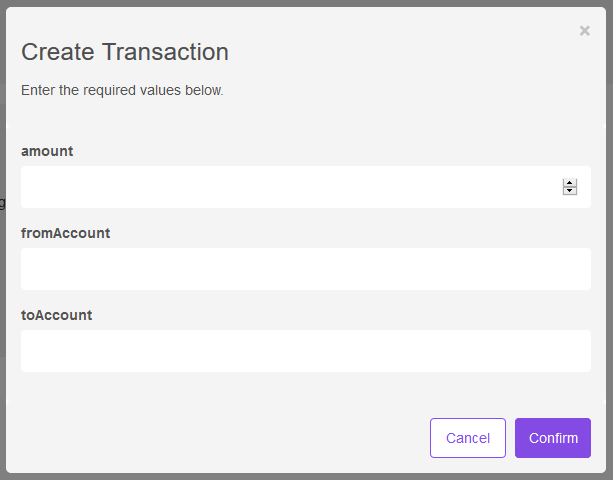
\includegraphics[width=0.3\textwidth]{Figures/webapp-transfer}
  \caption{\bf\small Credit/Debit Transfers }
  \label{fig:webapp-transfer}
\end{figure}

Assets may be changed directly with the appropriate permissions without facilitating any of the mentioned transactions in order to administer them. Regardless of the way of changing assets, thus, using custom transactions or just executing changes directly, all manipulations to the chain are recorded to the chain and clearly traceable.

In figure \ref{fig:webapp-transfer} the graphical interface for an invocation of a credit/debit transfer is illustrated. It is picking up a \textit{fromAccount}, \textit{toAccount} and a amount which is going to be transferred. As explained in section \ref{sec:chaincode}, for a \textit{DebitTransfer} to be performed, the owner of the \textit{fromAccount} needs to send a \textit{DebitTransferAcknowledge} confirmation.
\chapter{Conclusion and Final Thoughts}
\label{ch:conclusion}

\vspace{-1cm}
\begin{center}
Eduard Hirsch
\end{center}

This last chapter discusses the goals reached as well as the problems encountered during the development of the INTERLACE prototype. Additionally, it emphasises possible enhancements necessary and issues which need to be taken into account in order to bring the prototype to production level. Finally, it discusses parts that could not be finished as well as after-INTERLACE goals.

\section{Best Practices, Falsey Values and Pitfalls}

When using Hyperledger Composer but also when connecting to Hyperledger Fabric directly, it is important to pay attention to some points. Developers have to be aware that working with chaincode or smart contracts is quite different from accessing data as usual in a RDBMS,\footnote{Relational Database Management System} even though up-to-date frameworks shield a lot of the complexity underneath. Thus, even though access to the data structures and virtual machine/execution capabilities looks similar from a developer's point of view, it is necessary to account for some peculiarities related to blockchain-based technologies, because of their highly distributed nature. In the following sections we discuss and attempt to clarify some of these peculiarities.

\subsection{Deterministic Execution}

One of the most important things to keep in mind when writing chaincode applications is the deterministic execution of transactions. Although it seems quite obvious at first, it can be quite challenging to achieve.

One example is the \textbf{generation of IDs}: in a standard database environment simple locking mechanisms are in place to ensure correct primary keys for entries in a table. For blockchains which live in a distributed, consensus-based system it is problematic to create identifiers over chaincode execution. The reason is that each peer processing a transaction would compute a new ID completely independently, and most likely at the about the same time. Thus, if such a key-/ID-generation created different IDs on different clients, it might not be possible to reach consensus; thus, although nothing is actually wrong with the transaction itself, the resulting blockchain states in each peer would be different and therefore the last action would be rolled back. This would be especially hard to deal with during race conditions, and even more difficult to find out why a particular problem has occurred.

One solution to this problem could be to generate the ID from the client and pass it to the transaction as parameter. This would result in a much safer creation process which, additionally, is much faster during execution.

Another problem is posed by the use of \textbf{random numbers}. Since such calculations would reach different results on the various peers of the network,  creating random numbers in chaincode executions would cause sever problems when creating IDs from those numbers or randomizing decisions based on them, causing the results being indeterministic. Further, since it is not possible to know when a peer in the network will receive a new transaction, also the \textbf{creation of a date} or a timestamp contains an intrinsically random factor. Thus, dates created by different peer nodes during chaincode execution are prettly likely at least a bit different and when written into an e.g.\ asset are causing deviating blocks with different hashes of chains on the various nodes, and would therefore be rolled back when detected.

In listing \ref{lst:wrongDate} an example of a chaincode function is illustrated which creates a new date in line 8. The variable $currentDate$ will be filled with the current timestamp of the nodes Operating System.

\begin{center}
\begin{minipage}{0.8\textwidth}
\small
\begin{lstlisting}[language=javascript,firstnumber=1,caption={\bf\small An example of wrong determination of the current date inside of chain code}, captionpos=b,label=lst:wrongDate]
/**
 * CreditTransfer transaction
 * @param {net.sardex.interlace.CreditTransfer} transfer
 * @transaction
 */
async function CreditTransfer(transfer) {
  [...]
  let currentDate = new Date(); //incorrect!
  [...]
}
\end{lstlisting}
\end{minipage}
\end{center}

This implementation will lead as mentioned to inconsistent values of different peer nodes which may result in various problems.

For example, a possible scenario is that the date has been truncated to contain only day, month and year (no hour, seconds, ...), such that execution of the same transaction on different peers is likely to happen on the same day. In such a case, peers are able to reach consensus most of the time. However, validation of a transaction on different blockchain nodes would not be possible if it happens on different days (if e.g. execution is delayed or at the end of a day) or (re-)checked retroactively.

To explain further, chaincode running on peer $A$ may produce a date of 12 April 2018 at 23:59 in the evening. If peer node $B$ receives the same transaction at 00:00 the next day, it will produce the date 13 April 2018. Also, if e.g.\ somebody wants to check if the blockchain is in a consistent state, a transaction might be re-executed at any point in time after 12 April 2018 (staying with this example). Then the chaincode needs to run again and a date already written into the chain will be definitely different from the date produced during the re-execution. Consequently, those examples will lead to different outcomes on different peer nodes and therefore will trigger a rollback of the transaction or mark the whole chain as invalid from the point in time where that particular transaction had been appended to the ledger\footnote{Ledger structure: \url{https://hyperledger-fabric.readthedocs.io/en/release-1.3/ledger/ledger.html}}.

The solution to these kind of problems is to provide that possibly changing factor as an input parameter instead of creating it inside of the chaincode. Input parameters stay the same once a transaction proposal has been accepted and written into the chain. Thus, for every re-execution or validation they may be picked from there, allow re-run the code resulting in the same outcome every time when called. Therefore the re-generation of the the block hash will give the exact same hash like the "previous Hash" attribute of the the next block.

Given our Hyperledger Composer implementation the solution to the date problem could be to add an additional attribute for the abstract transaction $Transfer$ inside of our CTO-model definition, like adding $DateTime\ timeInitiated$. Then it would be necessary to pass a date value to the transaction for the $timeInitiated$ property when invoked by a client which then could be read from the transaction during chaincode processing.

However, in case of the date a better solution is offered by Hyperledger. When looking at the sequence diagram of the transaction flow\footnote{\url{https://hyperledger-fabric.readthedocs.io/en/release-1.3/arch-deep-dive.html\#swimlane}} which is prescribed by the Hyperledger protocol the very first step when proposing a transaction is to submit a $PROPOSE$ message to the endorsing peers which contain, beneath other things, the current timestamp which is further part of the transaction and finally stored into a block. Thus, the prototypical INTERLACE implementation is facilitating this timestamp to achieve the same goal like the propagation of the current date using the Transfer CTO-type. The code example in \ref{lst:correctDate} finally shows how the date may be read from the transaction.

\begin{center}
\begin{minipage}{0.8\textwidth}
\small
\begin{lstlisting}[language=javascript,firstnumber=1,caption={\bf\small An example of a correct determination of the current date inside of chain code}, captionpos=b,label=lst:correctDate]
/**
 * CreditTransfer transaction
 * @param {net.sardex.interlace.CreditTransfer} transfer
 * @transaction
 */
async function CreditTransfer(transfer) {
  [...]
  let currentDate = transfer.timestamp //correct!
  [...]
}
\end{lstlisting}
\end{minipage}
\end{center}


\textbf{Final note: Chaincode needs to be executed deterministically and has to reach, given its input parameters, the same result(s) on all the peer nodes at any point in time}. Consequently many parameters cannot be generated by chaincode directly but need to be provided as parameters to a transaction. But since this means that the parameters are creatable on the client-side only, it is also necessary to implement the corresponding logic in a way that prevents them from being used to fool the system or bring it into an inconsistent state.

\subsection{Network Upgrade}

Traditionally, updating a database after changes to the database model may be quite cumbersome due to the presence of new fields, foreign keys, and many other similar issues. However, various methods and strategies are in place for handling these issues.
On the other hand, since blockchains are usually spread over various peers that store replicated data, in contrast to traditional databases it is inherently more difficult to change the distributed structures to fit some new schema necessary to add a new feature or functionality.

Updating or changing values of asset attributes, as well as getting executable code and data structures ready for the next version of the network, may run into several problems. In particular, in order to maintain consistency and reliably achieve all fixes it is necessary to apply all changes to the network in such a way that upgrading the business network (CTO-File, chaincode, ...) and fixing the asset values happen in the right order, and while nobody else is able to interfere. This can be achieved by executing the upgrade as a single atomic transaction or, if that's not possible, by blocking common user access during deployment.

Thus, it is quite important to get everything right from the beginning, as it can be extremely difficult to apply certain changes. Consequently, it is highly advisable to think about possible changes and future scenarios together with possible side-effects and costs before first deployment to production systems.

\subsection{Hyperledger Composer Specifics}

Composer can be seen as a rapid-development approach. Its API sits on top of the Hyperledger Fabric framework. It tries to shield complexity from the user and aims to significantly reduce the time necessary to create distributed applications for Hyperledger Fabric.

For the development of the INTERLACE transactional service this meant that:
\begin{quote}
\vspace{-0.3cm}
\begin{itemize}
	\item models could be transferred easily,
	\item chaincode could be based on these models,
	\item a REST Server was supplied and
	\item a web-application generator was available.
\end{itemize}
\vspace{-0.3cm}
\end{quote}
Consequently, it was an ideal framework for prototyping. In addition, once a suitable cloud provider has been found, spinning up a network is straightforward. When hosting a network without an external provider who knows how to run these networks, much of the initial speed in creating it might be lost because, in such a case, a much deeper understanding of the whole architecture is necessary. Thus, also a greater effort is needed to get a ready implementation to work.

\textbf{Note:} For production systems it would be necessary to change to a plain Fabric implementation because Composer is still at quite an early stage of development, and there are even rumours that it may be discontinued. The reason is that some of the new features of the Fabric releases are deviating from the structures implemented by Composer. So it is becoming increasingly difficult for Hyperledger Composer developers to provide new features and functionalities available for Fabric.

\section{Identity Management}
\label{sec:id-management}

As mentioned in previous sections, we skipped Identity Management for the prototype in order to simplify the environment, decrease development efforts and therefore offer a relatively easier access to an example mutual credit system, hoping that this would make it easier to understand the basics. Nevertheless, it would be possible and quick to create additional participants and grant them access to the network in addition to just the currently used admin account. For example, an identity card can be issued for the first participant defined in transaction "InitBlockchain" which is identified by "m1". The example below illustrates how this might be done:

\begin{lstlisting}[language=bash]
	composer identity issue -c admin@tutorial-network -f m1.card -u m1 -a "resource:net.sardex.interlace.Individual#m1" -x true 
\end{lstlisting}
\vspace{-0.3cm}

This identity card is facilitated by the REST server and corresponds to a participant in the business network. 
But, when accessing the REST server, before a user can act with that identity it is necessary for him/her to log in first and authenticate his/her identity in some sort of way. To do so composer-rest-server uses an authentication middleware implemented in JavaScript called \textit{Passport.js}.\footnote{\url{http://www.passportjs.org/}}

The passport middleware offers many different authentication strategies and is quite a mature Open Source framework. An example of how to authenticate with OAuth and GitHub can be found on the Composer documentation website;\footnote{\url{https://hyperledger.github.io/composer/latest/integrating/enabling-rest-authentication}} but also different schemes can be used, like the JSON Web Tokens (JWT\footnote{\url{https://jwt.io/}}) which is mentioned in the issue tracker of the Hyperledger Composer GitHub page.\footnote{\url{https://github.com/hyperledger/composer/issues/2038}}

Passport is a commonly known middleware for authentication and may be applied also to different scenarios. Thus, it is usable well also if Composer is swapped for another technology.

\section{Future Scenarios}
\label{sec:future-scene}

Because we are using Hyperledger Fabric, extending the network is only a matter of changing the configuration. The approach taken for the INTERLACE prototype, shown in Figure \ref{fig:prototype-net-ext}, creates a new organisation for every payment circuit that deals with a new specific region. Consequently, each region would be responsible for hosting their own peers and ideally also their own certification authority (CA). However, certificates might be still handled by the Sardex CA. 

Sardex, in this scenario, is providing the network architecture and transferring the know-how about how to run a circuit, which would result in a model similar to a franchise. Although the clients and various other visible graphical interfaces may be branded in various ways, the underlying platform infrastructure would be predefined by Sardex in order to make the network work consistently.

The orderer will be handled by Sardex as well, but later might be handed over to an e.g.\ non-profit organisation representing the circuit and enforcing fair and clearly defined rules within a governance framework defined in collaboration with the circuit members themselves. To ensure a reliable system and a high performance throughput, an orderer could be clustered locally but also over various regionally separated areas.

\begin{figure}[htbp]
  \centering
  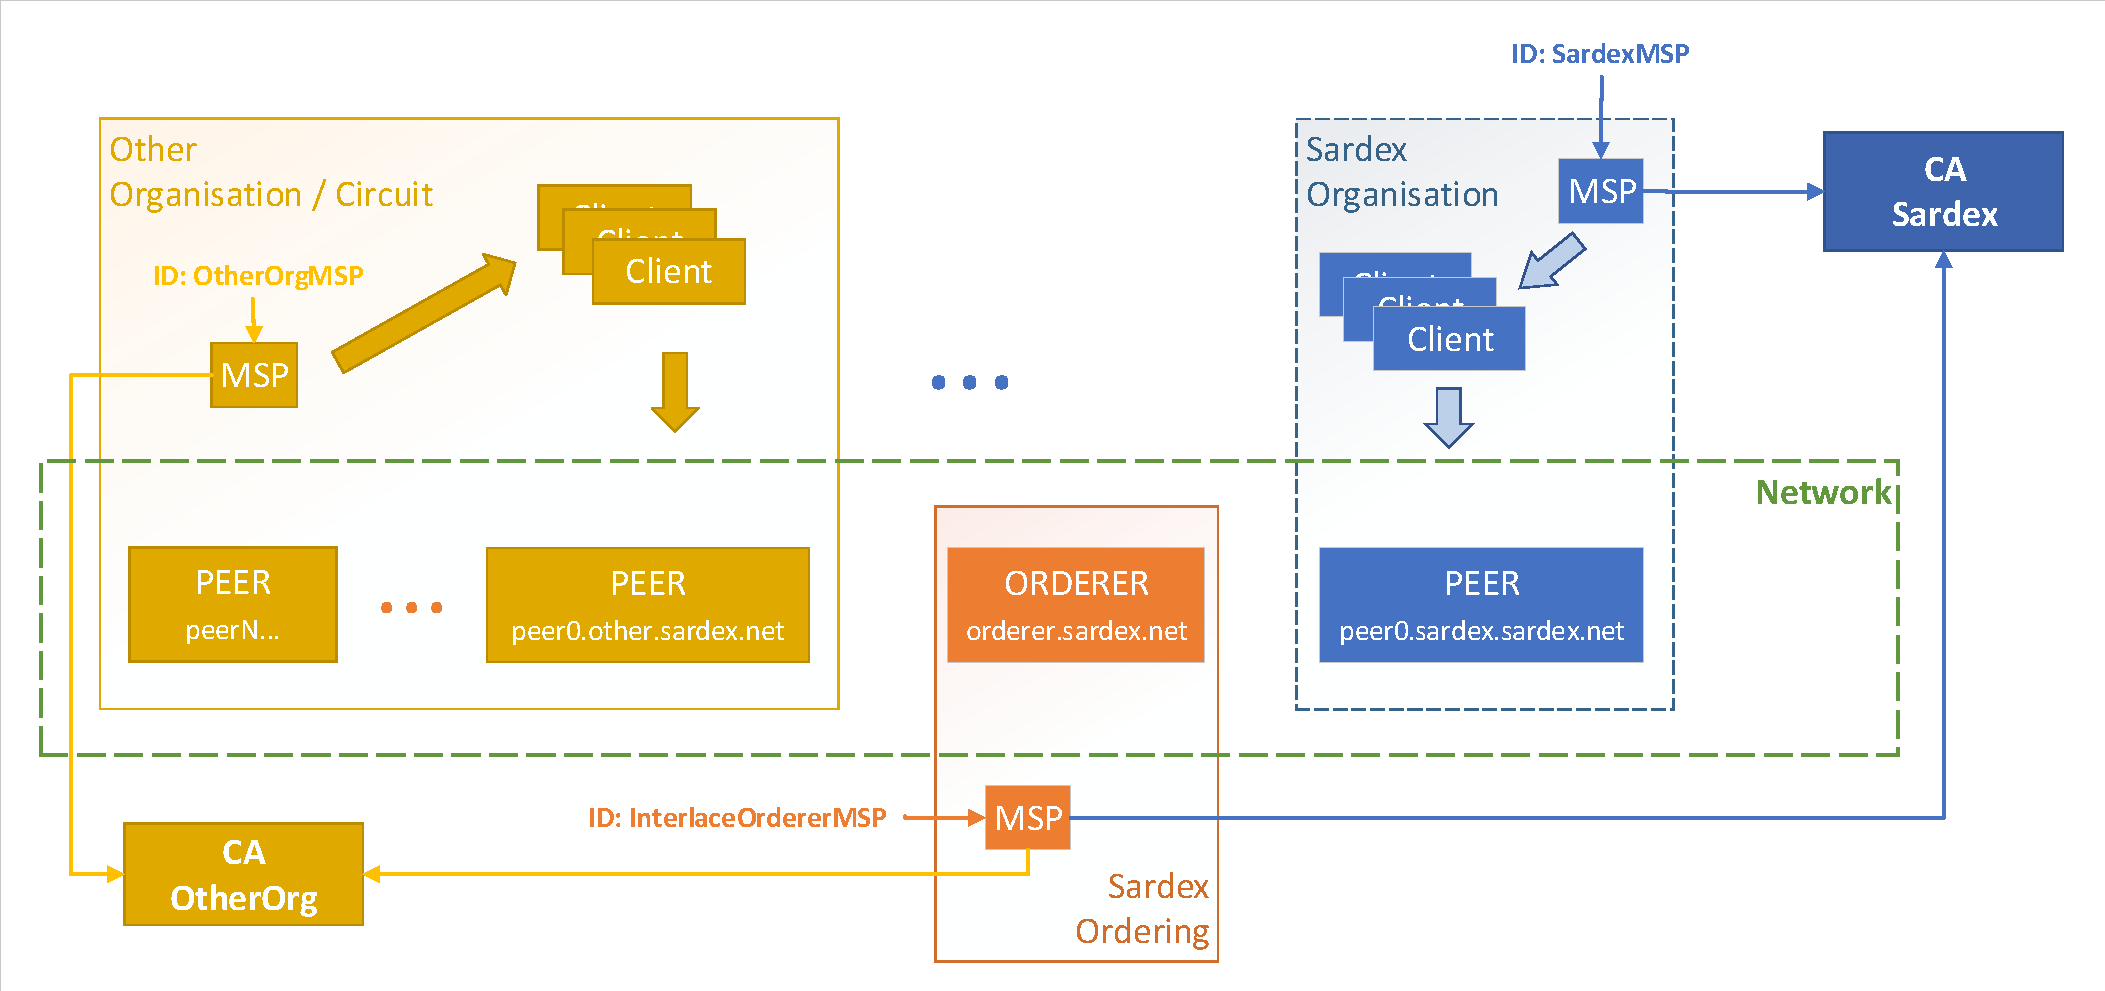
\includegraphics[width=1.0\textwidth, clip, trim=1mm 1mm 1mm 1mm]{Figures/extended-network}
  \caption{\bf\small Extended Network Structure}
  \label{fig:prototype-net-ext}
\end{figure}

\section{Final Review and Open Points}

Our DLT application prototype forms a stable and scalable basis for a reliable payment circuit. In fact, although the prototype was developed with Hyperledger Composer, which IBM may discontinue support for, any subsequent implementation in Hyperledger Fabric only will now be much easier to realize. This is also because newer versions of Fabric support a node.js SDK,\footnote{Software Development Kit} which would even allow the transfer of JavaScript code bits.

In summary, the goal of creating a reliable DLT has been achieved, and forms a necessary foundation for the various other services provided in future for the production-level business solutions created by and with Sardex.

\subsection{Open Points}

The \textbf{GDPR}\footnote{General Data Protection Regulation \cite{GDPR}} directive that came into effect in the first half of 2018 represents a challenge for blockchain solutions and, therefore, also for the INTERLACE project. It is necessary that personal information is not exposed to other parties unless necessary and unless it is done in agreement with its owners. In addition, each piece of information collected for the user or provided by the user needs to be deletable if the user requests it, and it must certainly be possible to look up upon request exactly what data was collected.

Information is reliably stored inside of a blockchain. Thus, looking up information is actually not an issue. Rather, one of the challenges is to keep it secret from being read by other parties, since standard blockchain approaches copy everything to every peer. Another challenge is the immutability of most blockchains, since GDPR enforces the right to be forgotten. The privacy aspect is solved currently by making the actual chain only accessible by the peers that are owned by the organisation running the local circuit. In this configuration, the clients that perform transfers have restricted access and cannot see the whole blockchain.

In later stages it may be possible for every business/party participating in the payment network to access the blockchain directly, i.e.\ to run a node. In this case the so-called \textit{SideDB}\footnote{\url{https://hyperledger-fabric.readthedocs.io/en/latest/private-data/private-data.html}} can be taken into consideration because it is a way offered by Hyperledger Fabric to store information which is only known by the respective client and only shared if permitted by the client.

\textit{SideDB} also solves the problem of GDPR-relevant data because, first, it is only exposed ``to whom it may concern'' and, second, it can be purged without making the chain invalid. The reason is that in SideDB only hashes of transactions and data are stored on the chain, which still makes it verifiable by regenerating the hash and comparing every time a datum needs to be verified. Normally the data only needs to be provided if specifically asked for, e.g.\ in case of an (external) audit.

The second point which needs further effort is the part of the testing coverage where the \textbf{ASIM implementations} are \textbf{tested} against the actual implementation of the prototype and later against the production-level implementation. These tests will be covered in deliverables D4.1 and D4.2 whose future versions will be completed after the end of the project.








%\input{2-DLTs_Selected/dlt}
%\input{3-Functional_Requirements/funreq}
\chapter*{References}
%\renewcommand{\section}[2]{}

\setlength{\parskip}{0.8\baselineskip}
\bibliographystyle{plainurl}
{\small
\addcontentsline{toc}{chapter}{References}
\bibliography{Bib/BioComp_References}}


%===================================================
%================== APPENDIX (1st way, used in D3.1)
%===================================================
%\appendix
%\addcontentsline{toc}{chapter}{Appendix: Complete Functional Requirements and Business Logic Model (2018)}
%\setcounter{chapter}{1}
%\renewcommand\thechapter{}
%\makeatletter
%\renewcommand\thesection{\@Alph\c@chapter.\@arabic\c@section}
%\makeatother
%\input{6-Appendix/SardexNewPaymentSpec_V6}


%===================================================
%================== APPENDIX (2nd way)
%===================================================
%\begin{appendix}
%\section*{Appendix}
%\includepdf[pages={-}]{sections/4-CaSM/CaCycleAsm.pdf}
%\end{appendix}

\end{document}
